\chapter{Ecuaciones en diferencias de orden 1}
En este tema, vamos a estudiar funciones de un intervalo $I \subseteq \bb{R}$ en $\bb{R}$.
\begin{itemize}
    \item Si $f$ es una recta, $f(x) = ax+b$, la ecuación se dice que es lineal.
    \item Si $f$ no es una recta, $x_{n+1} = f(x_n)$. No es una ecuación lineal. Se dice que no es lineal.
\end{itemize}

Algunos ejemplos de modelos que veremos son:
\begin{itemize}
    \item Modelo de la oferta y demanda (o Modelo de la Telaraña).
    \item Modelo logístico.
\end{itemize}

\section{Ecuación lineal de orden 1}
Una ecuación lineal general de orden 1 es una ecuación con forma:
$$x_{n+1} = ax_n + b_n$$
Con $a, b \in \bb{R}$ y $n \in \bb{N}$ (Aunque se podrían considerar $a, b \in \bb{C}$, en esta asignatura por norma general no lo consideraremos). Esta se denomina ecuación lineal completa.\\

A $x_{n+1} = ax_n$ se le llama la parte \textbf{homogénea} de la ecuación. Por tanto, una ecuación lineal homogénea será de la forma:
$$x_{n+1} = ax_n$$

\begin{definicion}[Ecuación autónoma]
    Una ecuación autónoma es una ecuación donde la dependencia del tiempo está vista a lo largo de la solución. Son del tipo:
    $$x_{n+1} = f(x_n)$$
\end{definicion}

Notemos que no todas las ecuaciones han de ser autónomas. Una ecuación no autónoma sería de la siguiente forma:
    $$x_{n+1} = f(x_n, n)$$
Con $f:\bb{R}\times\bb{N}\to \bb{R}$ Por tanto, la ecuación lineal general de orden 1 es una ecuación no autónoma, ya que el término independiente $b_n$ es una sucesión que depende del valor de $n$.

\subsection{Ecuación lineal de orden 1 autónoma}
En esta sección estudiaremos las ecuaciones lineales de orden 1 autónomas; es decir, el caso en el que $b_n = b~\forall n \in \bb{N}$. Su ecuación por tanto toma la siguiente forma:
$$x_{n+1} = ax_n + b$$
Vamos a estudiar dos formas de resolverla.

\subsubsection{Primera forma}
Iterando y buscando una expresión general para $x_n$. Dado $x_0$, tenemos que:
\begin{align*}
    x_1 &= ax_0 + b\\
    x_2 &= ax_1 + b = a(ax_0 +b)+b = a^2 x_0 + ab + b\\
    x_3 &= ax_2 + b = a(a^2x_0 + ab +b )+ b = a^3 x_0 + a^2b + ab + b\\
    \vdots&\\
    x_n &= a^n x_0 + a^{n-1} b + \ldots + b = a^n x_0 + b\sum_{k=0}^{n-1} a^k
\end{align*}
donde el valor de $x_n$ lo hemos obtenido de forma intuitiva. Demostrémoslo mediante inducción:
\begin{proof}
    Vamos a probar que la expresión general para la ecuación anterior es:
    $$x_n = a^n x_0 + a^{n-1} b + \ldots + b$$
    Por inducción:
    \begin{itemize}
        \item \ul{Caso base $n = 1$}:
        
        Para $n=1$, tenemos efectivamente $x_1=ax_0+b$.
        
        \item \ul{Supuesto para $n$, demostramos para $n+1$}:
        \begin{align*}
            x_{n+1} &= ax_n + b \AstIg\\
            &\AstIg a\left(a^n x_0 + a^{n-1} b + \ldots + b\right)+b =\\
            &= a^{n+1}x_0 + a^nb + \dots + ab + b
        \end{align*}
        donde en $(\ast)$ hemos aplicado la hipótesis de inducción.
    \end{itemize}
\end{proof}
Por tanto, hemos demostrado que en el PVI $x_{n+1} = ax_n + b$ se tiene que:
\begin{align*}
    x_n &= a^n x_0 + a^{n-1} b + \ldots + b
    =\\&= a^n x_0 + b(a^{n-1} + a^{n-1} + \ldots + a + 1)
    =\\&= a^n x_0 + b\sum_{k=0}^{n-1}a^k \AstIg a^n x_0 + b\cdot \dfrac{1-a^n}{1-a}
\end{align*}
donde en $(\ast)$ hemos usado el resultado de dicha suma de una serie geométrica.
Por tanto, la solución del problema de valores iniciales (PVI) descrito es:
            $$x_n = a^n x_0 + b\cdot \dfrac{1-a^n}{1-a}$$

\subsubsection{Segunda forma}
Si $b = 0$, sabríamos resolver la ecuación, ya que sería $x_{n+1} = ax_n$
y sus soluciones sabemos que son de la forma $x_n = a^n x_0$.
Por tanto, en este caso tratamos de buscar un cambio de variable para obtener una ecuación de ese tipo, que sí sabemos resolver. Buscamos un cambio de variable de la forma $y_n = x_n - k$ ($k \in \bb{C}$) tal que $y_n$ sea solución de la ecuación $y_{n+1} = ay_n$. Calculemos el valor de $k$:
$$y_{n+1} = x_{n+1} - k = ax_n + b - k \AstIg ay_n + ak + b - k$$
donde en $(\ast)$ he usado que $x_n = y_n + k$.
Como buscamos que $y_{n+1} = ay_n$, el valor de $k$ viene dado por la ecuación:
\begin{equation*}
    ak + b - k = 0 \Longleftrightarrow k = \frac{b}{1-a}
\end{equation*}

Por tanto, consideramos el cambio $y_n = x_n - \dfrac{b}{1-a}$, y tenemos que $y_{n+1} = ay_n$. La solución a dicha ecuación es conocida:
$$y_n = y_0\cdot a^n$$

Sabiendo esto, encontramos la solución del PVI:
\begin{align*}
    x_n &= y_{n} + k = y_n + \frac{b}{1-a} = y_0\cdot a^n + \frac{b}{1-a}
    =\\&= \left(x_0 - \frac{b}{1-a}\right)\cdot a^n + \frac{b}{1-a}
    =\\&= a^nx_0 + b\cdot \frac{1-a^n}{1-a}
\end{align*}
Como no podía ser de otra forma, hemos llegado a la misma solución que en el caso anterior.

\begin{observacion}
Notamos ahora que el $k$ encontrado es precisamente la solución constante de la ecuación $x_{n+1} = ax_n + b$.
\begin{equation*}
    c = ac + b \Longleftrightarrow c = \frac{b}{1-a} = x_c
\end{equation*}
\end{observacion}

\begin{observacion}
    Notemos que, siguiendo ambos métodos para resolver, llegamos a un problema para $a = 1$, ya que estaríamos dividiendo entre $0$. Pensamos ahora cómo solventar este problema.

    En este caso, simplemente, se nos queda una ecuación del estilo:
    $$x_{n+1} = x_n + b$$
    Su solución podemos pensar fácilmente que es la siguiente:
    $$x_n = x_0 + n\cdot b$$
    Notemos que la ecuación no tiene soluciones constantes, salvo que $b = 0$.
\end{observacion}

Por tanto, a modo de resumen, las soluciones de una ecuación lineal de primer orden autónoma son:
$$\left\{ \begin{array}{ll}
    \text{Si } a \neq 1: & x_n = \left( x_0 - \dfrac{b}{1-a} \right)a^n + \dfrac{b}{1-a} \\ \\
    \text{Si } a = 1: & x_n = x_0 + n \cdot b
\end{array}\right.$$

\subsubsection{Comportamiento de las soluciones a largo plazo}

En esta sección estudiaremos el comportamiento de las soluciones a largo plazo, también llamado comportamiento asintótico del modelo. Esto es cuando $n\to \infty$. Distinguimos en función del valor de $a$:

\begin{itemize}
    \item \ul{$|a| \neq 1$:}
    \begin{itemize}
        \item \ul{$|a| < 1$:}
        \begin{equation*}
            \lim_{n\to \infty} x_n 
            = \lim_{n\to \infty}\left( x_0 - \dfrac{b}{1-a} \right)a^n + \dfrac{b}{1-a} = \frac{b}{1-a}
        \end{equation*}
        \item \ul{$|a| > 1$:}
        \begin{itemize}
            \item $x_0 \neq \dfrac{b}{1-a}$:
                \begin{equation*}
                   x_n = \left( x_0 - \dfrac{b}{1-a} \right)a^n + \dfrac{b}{1-a}
                \end{equation*}
                En este caso, como $|a|>1$, tenemos que no converge.
            \item $x_0 = \dfrac{b}{1-a}$:
            \begin{equation*}
                    \lim_{n \to \infty} x_n = \lim_{n\to \infty}\left( x_0 - \dfrac{b}{1-a} \right)a^n + \dfrac{b}{1-a} = \lim_{n\to \infty} 0 + \dfrac{b}{1-a} = \dfrac{b}{1-a}
                \end{equation*}
        \end{itemize}
            
    \end{itemize}
    \item \ul{$|a| = 1$:}
    \begin{itemize}
        \item \ul{$a = 1$:}
        \begin{itemize}
            \item Si $b \neq 0$:
            
            Entonces, $x_n = x_0 + b \cdot n$
            \begin{equation*}
                \lim_{n \to \infty} |x_n| = \lim_{n \to \infty} |x_0+b\cdot n| = \infty
            \end{equation*}

            \item Si $b = 0$:
            Todas las soluciones son constantes.
        \end{itemize}
        \item \ul{$a = -1$:}

        \begin{equation*}
            x_n = \left(x_0-\frac{b}{2}\right)(-1)^n + \frac{b}{2}
        \end{equation*}
        \begin{itemize}
            \item $x_0 = \dfrac{b}{2}$:
            
            Tenemos que $x_n=\dfrac{b}{2}~ \forall n\in \bb{N}$. Es una solución constante.

            \item $x_0 \neq \dfrac{b}{2}$:
            
            Distinguimos el caso de los $n$ pares o impares:
            \begin{align*}
                x_{2n} &= \left(x_0-\frac{b}{2}\right)(-1)^{2n} + \frac{b}{2}
                = \left(x_0-\frac{b}{2}\right) + \frac{b}{2} = x_0\\
                x_{2n+1} &= \left(x_0-\frac{b}{2}\right)(-1)^{2n+1} + \frac{b}{2}
                = -\left(x_0-\frac{b}{2}\right) + \frac{b}{2} = b-x_0
            \end{align*}

            En este caso, tenemos que no converge en el infinito, y se trata de un $2-$ciclo.
        \end{itemize}

        \item \ul{$a \in \bb{C} \setminus \{ -1, 1\},~ |a| = 1$}:

        Como bien mencionamos, en esta asignatura solo consideraremos $a,b\in \bb{R}$. Se deja al lector el ejercicio de pensar qué ocurriría en este caso.
    \end{itemize}
\end{itemize}

\begin{ejercicio*}
    Estudia el comportamiento asintótico de:
    \begin{enumerate}
        \item $x_{n+1} = 2x_n + 5$

        En este caso, las soluciones son:
        \begin{equation*}
            x_n = \left(x_0+5\right)a^n -5
        \end{equation*}
        Como $|a|>1$, tenemos que no converge asintóticamente.
        
        \item $2x_{n+1}= x_n + 6$

        Tenemos que $x_{n+1}=\nicefrac{1}{2}x_n + 3$. Por tanto, como $|a|<1$, converge a $\dfrac{3}{\nicefrac{1}{2}}=6$.
    \end{enumerate}
\end{ejercicio*}

\subsection{Ecuación lineal de orden 1 no autónoma}
$$x_{n+1} = ax_n + b_n$$
Es la ecuación lineal no autónoma, donde $b_n$ es una sucesión. La función asociada es $f(x,n) = ax + b_n$, de forma que:
$$x_{n+1} = f(x_n, n)$$

Vamos a estudiar las formas de resolver la ecuación. 

\subsubsection{Conociendo una solución particular}
Si conocemos $\overline{x_n}$ una solución particular de la ecuación, entonces aplicamos el cambio de variable
$$y_n = x_n - \overline{x_n}$$

De esta forma, nos queda que:
\begin{equation*}
    y_{n+1} = x_{n+1} - \ol{x_{n+1}}
    = ax_n + b_n - \ol{x_{n+1}} = ax_n - a\ol{x_n} = ay_n
\end{equation*}

Por tanto, como dicha ecuación sí sabemos resolverla, tenemos que:
$$x_n = y_n + \ol{x_n} = y_0 a^n + \ol{x_n} = \left(x_0-\ol{x_0}\right)a^n - \ol{x_n}$$

Veamos ahora algunos ejemplos de resolución de ecuaciones lineales de orden 1 no autónomas:
\begin{ejercicio*}
    Consideramos la ecuación lineal no autónoma dada por:
    \begin{equation*}
        x_{n+1} = \frac{x_n}{2} + n\qquad \forall n \in \bb{N}
    \end{equation*}
    Resuélvela siguiendo los siguientes pasos:
    \begin{enumerate}
        \item ¿Tiene soluciones constantes?

        Sea $c\in\bb{R}$ una solución constante, entonces verifica que:
        \begin{equation*}
            c = \dfrac{c}{2}+n \Longrightarrow \dfrac{c}{2} = n \Longrightarrow c = 2n \quad \forall n \in \bb{N}
        \end{equation*}
        Como $c$ no puede ser igual a todos los naturales pares al mismo tiempo, tenemos que no hay soluciones constantes.
        
        \item Determina $\alpha,\beta\in \bb{R}$, para que $\ol{x_n}=\alpha n+\beta$ sea una solución particular.\\

        Como es una solución particular, para todo $n\in \bb{N}$ tenemos que:
        \begin{align*}
            \ol{x_{n+1}} = \frac{\ol{x_n}}{2} + n & \Longrightarrow 
            \alpha(n+1) + \beta = \frac{\alpha n + \beta}{2} + n \Longrightarrow \\&\Longrightarrow
            2\alpha n +2\alpha + 2\beta = \alpha n +\beta + 2n
            \Longrightarrow \\&\Longrightarrow
            \alpha n +2\alpha +\beta = 2n
        \end{align*}

        Tomando $n=1,2$, tenemos el siguiente sistema:
        \begin{equation*}
            \left\{\begin{array}{ll}
                3\alpha + \beta &= 2\\
                4\alpha + \beta &= 4
            \end{array}\right\}
            \Longrightarrow
            -\alpha = -2 \Longrightarrow
            \left\{\begin{array}{l}
                \alpha = 2\\
                \beta = -4
            \end{array}\right.
        \end{equation*}

        Por tanto, $\ol{x_{n}}=2n -4$ es una solución particular.
        
        \item Demuestra que $y_n:=x_n-\ol{x_n}$ es solución de una ecuación homogénea.

        Tenemos que:
        \begin{align*}
            y_{n+1} &= \frac{x_n}{2} + n - [2(n+1)-4]
            = \frac{x_n}{2} -n +2
            = \frac{x_n}{2} -(n-2)
            =\\&= \frac{x_n}{2} - \frac{2n-4}{2}
            = \frac{x_n-\ol{x_n}}{2}
            = \frac{y_n}{2}
        \end{align*}

        Por tanto, se trata de una ecuación homogénea, y tenemos por tanto que:
        \begin{equation*}
            y_n = \left(\frac{1}{2}\right)^ny_0
            = (x_0 - \ol{x_0})\left(\frac{1}{2}\right)^n
            = \frac{x_0+4}{2^n}
        \end{equation*}
        
        \item Encuentra todas las soluciones de la ecuación.

        Tenemos que:
        \begin{equation*}
            x_n = y_n + \ol{x_n}
            = \frac{x_0+4}{2^n} + 2n-4
        \end{equation*}
    \end{enumerate}
\end{ejercicio*}

\begin{ejercicio*}
    Consideramos la ecuación lineal no autónoma dada por:
    \begin{equation*}
        x_{n+1} = \frac{x_n}{2} + 2^n\qquad \forall n \in \bb{N}
    \end{equation*}
    Resuélvela siguiendo los siguientes pasos:
    \begin{enumerate}
        \item ¿Tiene soluciones constantes?

        Sea $c\in\bb{R}$ una solución constante, entonces verifica que:
        \begin{equation*}
            c = \dfrac{c}{2}+2^n \Longrightarrow \dfrac{c}{2} = 2^n \Longrightarrow c = 2^{n+1}\quad \forall n \in \bb{N}
        \end{equation*}
        Como $c$ no puede ser igual a distintos números al mismo tiempo, tenemos que la ecuación en diferencias no presenta soluciones constantes.
        \item Determina $\alpha\in \bb{R}$, para que $\ol{x_n}=\alpha 2^n$ sea una solución particular.\\

        Como es una solución particular, para todo $n\in \bb{N}$ tenemos que:
        \begin{align*}
            \ol{x_{n+1}} = \frac{\ol{x_n}}{2} + 2^n & \Longrightarrow 
            \alpha 2^{n+1} = \alpha 2^{n-1} + 2^n \Longrightarrow \\&\Longrightarrow
            \alpha (2^{n+1} - 2^{n-1}) = 2^n
            \Longrightarrow \\&\Longrightarrow
            \alpha = \dfrac{2^n}{2^{n+1}-2^{n-1}} 
            \Longrightarrow \\&\Longrightarrow
            \alpha = \dfrac{1}{2-\nicefrac{1}{2}} = \dfrac{2}{3}
        \end{align*}

        Por tanto, $\ol{x_n} = \frac{2}{3}\cdot 2^n$ es una solución particular.
        
        \item Demuestra que $y_n:=x_n-\ol{x_n}$ es solución de una ecuación homogénea.
        \begin{align*}
            y_{n+1} &= x_{n+1} - \dfrac{2}{3}2^{n+1} = \dfrac{1}{2}x_n + 2^n - \dfrac{2}{3}2^{n+1}
            = \frac{1}{2}x_n + 2^n\left(1-\frac{4}{3}\right)=\\
            &= \frac{1}{2}x_n - \frac{2^n}{3}
            = \frac{1}{2}x_n - \frac{2\cdot 2^n}{2\cdot 3}
            =\dfrac{1}{2}(x_n-\ol{x_n})
            = \dfrac{1}{2}y_n 
        \end{align*}

        Por tanto, se trata de una ecuación homogénea, y tenemos por tanto que:
        \begin{equation*}
            y_n = \left(\frac{1}{2}\right)^ny_0
            = (x_0 - \ol{x_0})\left(\frac{1}{2}\right)^n
            = \frac{x_0-\frac{2}{3}}{2^n}
        \end{equation*}
        
        \item Encuentra todas las soluciones de la ecuación.

        Tenemos que:
        \begin{equation*}
            x_n = y_n + \ol{x_n}
            = \frac{x_0-\frac{2}{3}}{2^n} + \frac{2}{3}\cdot 2^n
            = \frac{1}{2^n}\left(x_0 - \frac{2}{3}\right)+\frac{2^{n+1}}{3}
        \end{equation*}
    \end{enumerate}
\end{ejercicio*}

\begin{ejercicio*}
    Consideramos la ecuación lineal no autónoma dada por:
    \begin{equation*}
        x_{n+1} = \frac{x_n}{2} + \frac{1}{2^n}
    \end{equation*}
    Resuélvela siguiendo los siguientes pasos:
    \begin{enumerate}
        \item ¿Tiene soluciones constantes?\\
         Sea $c\in\bb{R}$ una solución constante, entonces verifica que:
        \begin{equation*}
            c = \dfrac{c}{2}+\dfrac{1}{2^n} \Longrightarrow \dfrac{c}{2} = \dfrac{1}{2^n} \Longrightarrow c = \dfrac{1}{2^{n-1}}\quad \forall n \in \bb{N}
        \end{equation*}
        Como $c$ no puede ser igual a distintos números al mismo tiempo, tenemos que la ecuación en diferencias no presenta soluciones constantes.
        
        \item Determina $\alpha\in \bb{R}$, para que $\ol{x_n}=\alpha n\cdot\frac{1}{2^n}$ sea una solución particular.\\

        Como es una solución particular, para todo $n\in \bb{N}$ tenemos que:
        \begin{multline*}
            \ol{x_{n+1}} = \frac{\ol{x_n}}{2} + \frac{1}{2^n} \Longrightarrow 
            \alpha (n+1)\cdot \frac{1}{2^{n+1}} = \frac{\alpha n}{2^{n+1}} + \frac{1}{2^n}
            \Longrightarrow \\ \Longrightarrow \alpha(n+1) = \alpha n + 2
            \Longrightarrow \alpha = 2
        \end{multline*}

        Por tanto, $\ol{x_n} = 2n\cdot \frac{1}{2^n} = \frac{n}{2^{n-1}}$ es una solución particular.
        
        \item Demuestra que $y_n:=x_n-\ol{x_n}$ es solución de una ecuación homogénea.
        \begin{align*}
            y_{n+1} &= x_{n+1} - \dfrac{n+1}{2^n} = \dfrac{1}{2}x_n + \frac{1}{2^n} - \dfrac{n+1}{2^n}
            = \frac{1}{2}x_n + \frac{1}{2^n}\left(1-(n-1)\right)=\\
            &= \frac{1}{2}x_n - \frac{n}{2^n}
            = \frac{1}{2}x_n - \frac{n}{2\cdot 2^{n-1}}
            =\dfrac{1}{2}(x_n-\ol{x_n})
            = \dfrac{1}{2}y_n 
        \end{align*}

        Por tanto, se trata de una ecuación homogénea, y tenemos por tanto que:
        \begin{equation*}
            y_n = \left(\frac{1}{2}\right)^ny_0
            = (x_0 - \ol{x_0})\left(\frac{1}{2}\right)^n
            = \frac{x_0}{2^n}
        \end{equation*}
        
        \item Encuentra todas las soluciones de la ecuación.

        Tenemos que:
        \begin{equation*}
            x_n = y_n + \ol{x_n}
            = \frac{x_0}{2^n} + \frac{n}{2^{n-1}}
        \end{equation*}
    \end{enumerate}
\end{ejercicio*}

\section{Modelo de la oferta y la demanda (o Modelo de la Telaraña)}
Suponemos que la oferta y la demanda son funciones que dependen del precio. Las notamos por:
\begin{itemize}
    \item Sea $D(p)$ la demanda en función del precio $p$.
    \item Sea $O(p)$ la oferta en función del precio $p$.
\end{itemize}

En función del precio $p$, es lógico pensar que la demanda debe ser decreciente y la oferta creciente. Esto se debe a que, conforme el precio aumenta, los clientes tendrán menor interés por comprar el producto; mientras que las empresas querrán venderlo más. Para simplificar, supondremos que son rectas:
\begin{align*}
    D(p) &= a-bp \qquad a,b \in \bb{R}^+\\
    O(p) &= c + dp \qquad d \in \bb{R}^+,~c\in \bb{R}
\end{align*}
A $b$ y a $d$ se les llama \textbf{marginal de demanda} y \textbf{marginal de la oferta}, respectivamente.
En los siguientes casos, tratamos de buscar un precio de equilibrio del mercado.

\subsection{Sistema estático}
En este caso, suponemos que $D(p) = O(p)$. Este es un caso ideal, ya que toda la demanda es cubierta por la oferta. Se busca el precio de equilibrio, que es el que permite que se dé este caso, y es el que se mantendrá constante para que la demanda se siga cubriendo. 
\begin{equation*}
    D(p)=O(p) \Longleftrightarrow
    a - bp = c+dp
    \Longleftrightarrow p_{equilibrio} = \dfrac{a-c}{b+d}
\end{equation*}
Para que esto tenga sentido (obtengamos un precio de equilibrio positivo), necesitamos que $a > c$.

\subsection{Sistema dinámico}
En este caso el precio va cambiando, por lo que se considera una sucesión $p_n$, que representa el precio en el periodo $n$. Se supone que para la oferta se considera con el precio del periodo $p_{n-1}$ y la demanda con $p_n$. Es decir, se intenta prever la demanda que va a haber en función de la oferta que había en el periodo anterior.
\begin{equation*}
    O(p_{n-1}) = D(p_n) \Longleftrightarrow
    c + dp_{n-1} = a-bp_n \Longleftrightarrow
    p_n = \dfrac{a-c}{b}-\dfrac{d}{b}\cdot p_{n-1}
\end{equation*}
Esta es una ecuación lineal de orden 1 autónoma, por ser el término independiente una constante. \underline{La solución constante del modelo}, denominada \ul{precio de equilibro} y notada por $p_e$ es $p_e=\dfrac{a-c}{b+d}$, veámoslo:
\begin{equation*}
    p_e = \dfrac{a-c}{b}-\dfrac{d}{b}p_e \Longleftrightarrow
    bp_e = a-c -dp_e \Longleftrightarrow
    p_e = \frac{a-c}{b+d}
\end{equation*}

Por tanto, la solución de dicha ecuación es:
$$p_n = (p_0 - p_e)\left(\dfrac{-d}{b}\right)^n + p_e $$

\subsubsection{Precio a largo plazo}
\begin{itemize}
    \item $0<\dfrac{d}{b}<1$:
    \begin{equation*}
        \lim_{n\to \infty} p_n = \lim_{n\to \infty} \left[(p_0 - p_e)\left(\dfrac{-d}{b}\right)^n + p_e \right]= p_e
    \end{equation*}
    
    Entonces, el precio tiende al precio de equilibrio, y lo hace oscilando (ya que tenemos un negativo elevado a $n$, a veces se le suma un precio o se le resta, aunque finalmente tiende a $0$).
    Esto ocurre cuando la marginal de la oferta, $d$ es menor que la marginal de la demanda, $b$. Esto es, cuando la oferta crece más lenta que la demanda.

    \item $1<\dfrac{d}{b}$:

    Entonces, la ecuación deja de tener sentido, porque toma valores negativos.

    \begin{equation*}
        \lim_{n\to\infty} |p_n| = \infty
    \end{equation*}

    \item $b=d$:

    Entonces, $p_n = (p_0 - p_e)\left(-1\right)^n + p_e$. Como hemos visto anteriormente, se trata de un $2-$ciclo.
\end{itemize}

Veamos ahora por qué se conoce como modelo de la telaraña. Supuesto $d<b$, hemos visto que el precio converge al precio de equilibrio. Veamos gráficamente qué implica esto:
\begin{figure}[H]
    \centering
    \begin{tikzpicture}
        \begin{axis}[
            axis lines = center,
            xlabel = $p$,
            legend pos=outer north east
        ]
        
        % Curva de oferta
        \addplot[domain=-1:10, samples=100, color=red]{2+0.5*x}; 
        \addlegendentry{$O(p)$}
        
        % Curva de demanda
        \addplot[domain=-1:10, samples=100, color=blue]{8 - 0.8*x}; 
        \addlegendentry{$D(p)$}
        
        % Trayectoria de la telaraña
        \draw[dashed, -stealth] (2, 3) -- (6.25, 3);
        \draw[dashed, -stealth] (6.25, 3) -- (6.25, 5.125);
        \draw[dashed, -stealth] (6.25, 5.125) -- (3.59375, 5.125);
        \draw[dashed, -stealth] (3.59375, 5.125) -- (3.59375, 3.796875);
        \draw[dashed, -stealth] (3.59375, 3.796875) -- (5.25390625,3.796875);
        \draw[dashed, -stealth]  (5.25390625,3.796875) -- (5.25390625,4.62695315);
        \draw[dashed, -stealth]  (5.25390625, 4.62695315) -- (4.21630859375, 4.62695315);
        \addlegendentry{Telaraña}
        \end{axis}
    \end{tikzpicture}
    \caption{Representación del modelo de la Telaraña.}
\end{figure}
Como podemos ver, el precio va convergiendo a al precio de equilibro en forma de telaraña, de ahí el nombre.

\section{Ecuación no lineal de orden 1}
En esta sección, estudiaremos buscar soluciones para ecuaciones de la forma:
\Func{f}{I\subseteq \bb{R}}{I\subseteq \bb{R}}{x_{n}}{f(x_n)=x_{n+1}}
con $I$ un intervalo de $\bb{R}$ y con $f$ no lineal. Es decir, no es de la forma: $f(x) = ax +b$. Recordamos que en la introducción vimos un modelo en esta familia, el modelo logístico, introducido en la Sección \ref{sec:IntroModeloLogistico} y desarrollado en la Sección \ref{sec:DesarrolloModeloLogistico}.
\begin{equation*}
    p_{n+1} = p_n(a-bp_n)
\end{equation*}

En general, no podemos encontrar una solución de forma general. En estos casos, debemos ver cómo se comportan las soluciones en torno a las soluciones que conocemos de forma sencilla. Recordamos que hay dos tipos de soluciones que suelen ser más fáciles de encontrar, que son:
\begin{itemize}
    \item Las soluciones constantes: $x_c\equiv c = \{c, c, \ldots \}$ es solución si $c$ es un punto fijo de $f$.
    \item Los ciclos: 
    $x_0$ genera un $n-$ciclo si $x_0$ es un punto fijo de $f^n=\overbrace{f\circ f \circ \ldots \circ f}^{n}$. Luego: $x_n = f^n(x_0) = x_0$.
\end{itemize}


\subsection{Puntos de equilibrio}
\begin{ejemplo}
    Sea la ecuación dada por el PVI:
    \begin{equation*}
    \left\{ \begin{array}{l}
        x_{n+1} = \dfrac{4}{x_n} \\
        x_0 > 0
    \end{array}\right.
    \end{equation*}
    Tenemos que no es lineal, ya que su función asociada es:
    \Func{f}{\bb{R}^\ast}{\bb{R}^\ast}{x}{\dfrac{4}{x}}

    Tenemos que el sistema es siempre un $2-$ciclo, para cualquier valor de $x_0 \in \bb{R}^+$:
    \begin{align*}
        x_1 &= \frac{4}{x_0}\\
        x_2 &= \frac{4}{x_1} = \frac{4}{\frac{4}{x_0}}=x_0
    \end{align*}

    Por tanto, $x_n$ es el $2-$ciclo $\{x_0, \nicefrac{4}{x_0}, \dots\}$.
    En el caso particular de que $x_0=2$, el $2-$ciclo es el ciclo trivial $x\equiv 2 = \{2,2,\ldots\}$; es decir, es una solución constante.
\end{ejemplo}

\begin{ejemplo}
Sea la ecuación dada por el PVI:
    \begin{equation*}
    \left\{ \begin{array}{l}
        x_{n+1} = x_n^2 \\
        x_0 \text{ dada}
    \end{array}\right.
    \end{equation*}
    Tenemos que no es lineal, ya que su función asociada es:
    \Func{f}{\bb{R}}{\bb{R}}{x}{x^2}

    Tenemos que:
    \begin{align*}
        x_1 &= x_0^2\\
        x_2 &= x_1^2 = x_0^4\\
        x_3 &= x_2^2 = x_0^8
    \end{align*}

    Por tanto, deducimos que el término general es (hágase la inducción):
    \begin{equation*}
        x_n = x_0^{(2^n)}
    \end{equation*}

    Las soluciones constantes tenemos que son:
    \begin{equation*}
        x\equiv 0 \qquad x\equiv 1
    \end{equation*}
    
    Usando conocimientos de límites, tenemos que:
    \begin{itemize}
        \item Si $|x_0|<1$:
        \begin{equation*}
            \lim_{n\to \infty}x_n = \lim_{n\to \infty} x_0^{(2^n)} = 0
        \end{equation*}
        \item Si $|x_0|>1$:
        \begin{equation*}
            \lim_{n\to \infty}x_n = \lim_{n\to \infty} x_0^{(2^n)} = \infty
        \end{equation*}
    \end{itemize}    
\end{ejemplo}

\begin{ejemplo}
    Sea la ecuación dada por el PVI:
    \begin{equation*}
    \left\{ \begin{array}{l}
        x_{n+1} = \sqrt{x_n} \\
        x_0 >0
    \end{array}\right.
    \end{equation*}
    Tenemos que no es lineal, ya que su función asociada es:
    \Func{f}{\bb{R}^+}{\bb{R}^+}{x}{\sqrt{x}}

    Tenemos que:
    \begin{align*}
        x_1 &= \sqrt{x_0}\\
        x_2 &= \sqrt{x_1} = \sqrt[4]{x_0}\\
        x_3 &= \sqrt{x_2} = \sqrt[8]{x_0}
    \end{align*}

    Por tanto, deducimos que el término general es (hágase la inducción):
    \begin{equation*}
        x_n = \sqrt[2^n]{x_0}
        =x_0^{\frac{1}{2^n}}
    \end{equation*}

    Las soluciones constantes tenemos que son:
    \begin{equation*}
        x\equiv 0 \qquad x\equiv 1
    \end{equation*}

    Usando conocimientos de límites, para $x_0\neq 0$, tenemos que:
    \begin{equation*}
        \lim_{n\to \infty}x_n = \lim_{n\to \infty} x_0^{\frac{1}{2^n}}=1
    \end{equation*}
    
    En el caso de $x_0 = 0$, ya hemos visto anteriormente que es una solución constante.
\end{ejemplo}

El caso anterior se podría haber probado sin necesidad de obtener el término general, como se puede ver en el siguiente ejemplo, más bien teórico.
\begin{ejemplo}[Genérico]
    Sea la ecuación dada por el PVI:
    \begin{equation*}
    \left\{ \begin{array}{l}
        x_{n+1} = f(x_n) \\
        x_0 \text{\ dado}
    \end{array}\right.
    \end{equation*}
    \Func{f}{]x_1^\ast, +\infty[}{]x_1^\ast, +\infty[}{x}{f(x)}

    Con $f$ continua, estrictamente creciente y con dos puntos fijos: $x_1^\ast$ y $x_2^\ast$, con $x_1^\ast < x_2^\ast$. Además, sabemos que:
    \begin{itemize}
        \item Si $x\in~]x_1^\ast, x_2^\ast[$, se tiene que $x < f(x)$.

        \item Si $x\in~]x_2^\ast, +\infty[$, se tiene que $f(x) < x$.
    \end{itemize}
    Estudiar cómo se comporta la ecuación en diferencias cuando $n\to \infty$.

    \begin{proof}
        Distinguimos en función del valor inicial $x_0$.
    \begin{itemize}
        \item Supongamos $x_1^\ast < x_0 < x_2^\ast$:

        Como $x_1^\ast < x_0 < x_2^\ast$ y $f$ es creciente, tenemos que:
        \begin{equation*}
            x_1^\ast=f(x_1^\ast) \leq f(x_0)=x_1 \leq f(x_2^\ast) = x_2^\ast
        \end{equation*}
        Por inducción (hágase) se demuestra que $x_1^\ast < x_n < x_2^\ast$ para todo $n\in \bb{N}$. Por tanto, $x_2^\ast$ es un mayorante de la sucesión $\{x_n\}$.
        
        Veamos ahora que la sucesión $\{x_n\}$ es creciente: $x_n < x_{n+1}$. Como $x_n \in ]x_1^\ast, x_2^\ast[$, se tiene que             $x_n < f(x_n) = x_{n+1}$ para todo $n\in \bb{N}$.

        Por tanto, como $\{x_n\}$ es creciente y mayorada, tenemos que es convergente. Supongamos que $\{x_n\}\to x\in \bb{R}$. Tenemos que:
        \begin{equation*}
            x_{n+1} = f(x_n)
            \Longrightarrow
            x = \lim_{n\to \infty} x_{n+1} 
            = \lim_{n\to \infty}
            f(x_n) = f\left(\lim_{n\to \infty}x_n\right) = f(x)
        \end{equation*}
        donde he empleado que $f$ es continua. Por tanto, como $f(x)=x$, tenemos que el límite $x$ es un punto fijo de $f$. Como la sucesión es creciente, tenemos que $x=x_2^\ast$, por lo que $\{x_n\}\to x_2^\ast$.

        \item Supongamos $x_2^\ast<x_0$:

        Como $x_2^\ast<x_0$ y $f$ es creciente, tenemos que:
        \begin{equation*}
            x_2^\ast=f(x_2^\ast) \leq f(x_0)=x_1
        \end{equation*}
        Por inducción (hágase) se demuestra que $x_2^\ast < x_n$ para todo $n\in \bb{N}$. Por tanto, $x_2^\ast$ es un minorante de la sucesión $\{x_n\}$.
        
        Veamos ahora que la sucesión $\{x_n\}$ es decreciente: $x_n > x_{n+1}$. Como $x_n \in ]x_2^\ast, +\infty[$, se tiene que
        $x_n > f(x_n) = x_{n+1}$ para todo $n\in \bb{N}$.

        Por tanto, como $\{x_n\}$ es decreciente y minorada, tenemos que es convergente. Supongamos que $\{x_n\}\to x\in \bb{R}$. Tenemos que:
        \begin{equation*}
            x_{n+1} = f(x_n)
            \Longrightarrow
            x = \lim_{n\to \infty} x_{n+1} 
            = \lim_{n\to \infty}
            f(x_n) = f\left(\lim_{n\to \infty}x_n\right) = f(x)
        \end{equation*}
        donde he empleado que $f$ es continua. Por tanto, como $f(x)=x$, tenemos que el límite $x$ es un punto fijo de $f$. Como un punto fijo suyo es $x_2^\ast$ y ya es un minorante, tenemos que $x=x_2^\ast$, por lo que $\{x_n\}\to x_2^\ast$.
    \end{itemize}

    Por tanto, hemos demostrado que $\{x_n\}\to x_2^\ast$.
    \end{proof}
\end{ejemplo}~\\

Veamos ahora qué ocurre si no hay dos puntos fijos, sino que tan solo hay uno.
\begin{ejercicio*}
    Fijado $a\in \bb{R}^+$, sea la ecuación dada por el PVI:
    \begin{equation*}
    \left\{ \begin{array}{l}
        x_{n+1} = \sqrt{x_n+a} \\
        x_0 \geq -a
    \end{array}\right.
    \end{equation*}

    Tenemos que no es lineal, ya que su función asociada es:
    \Func{f}{[-a, \infty[}{[0, \infty[}{x}{\sqrt{x+a}}

    Veamos los primeros términos de la sucesión:
    \begin{align*}
        x_1 &= \sqrt{x_0+a}\\
        x_2 &= \sqrt{x_1+a} = \sqrt{\sqrt{x_0+a}+a} \\
        x_3 &= \sqrt{x_2+a} = \sqrt{\sqrt{\sqrt{x_0+a}+a}+a}
    \end{align*}

    Por tanto, no es fácil encontrar un término general de la sucesión. Busquemos cuántos puntos fijos tiene:
    \begin{equation*}
        x = \sqrt{x+a} \Longleftrightarrow x^2=x+a \Longleftrightarrow
        x^2-x-a = 0 \Longleftrightarrow x=\frac{1\pm \sqrt{1+4a}}{2}
    \end{equation*}

    Consideremos $x_1^\ast=\dfrac{1-\sqrt{1+4a}}{2}$. Tenemos que:
    \begin{align*}
        x_1 = \frac{1-\sqrt{1+4a}}{2} < 0 &\Longleftrightarrow
        1 < \sqrt{1+4a} \Longleftrightarrow 1 < 1+4a
        \Longleftrightarrow 0<a
    \end{align*}
    Por tanto, tenemos que $x_1^\ast$ no es una solución. Es decir, tan solo hay una solución constante, $x_2^\ast=\dfrac{1+\sqrt{1+4a}}{2}$.
    Para ver su comportamiento en el infinito, distinguimos en función del valor inicial $x_0$.
    \begin{itemize}
        \item Supongamos $-a \leq x_0 < x_2^\ast$:

        Como $-a \leq x_0 < x_2^\ast$ y $f$ es creciente, tenemos que:
        \begin{equation*}
            0= f(-a) \leq f(x_0)=x_1 \leq f(x_2^\ast) = x_2^\ast
        \end{equation*}
        Por inducción (hágase) se demuestra que $0 < x_n < x_2^\ast$ para todo $n\in \bb{N}^\ast$. Por tanto, $x_2^\ast$ es un mayorante de la sucesión $\{x_n\}$.
        
        Veamos ahora que la sucesión $\{x_n\}$ es creciente: $x_n < x_n < x_{n+1}$. Se tiene que:
        \begin{equation*}
            x_n < x_{n+1} = \sqrt{x_n +a} \Longleftrightarrow x_n^2 < x_n +a
            \Longleftrightarrow x_n^2 - x_n -a <0
        \end{equation*}
        Como $a>0$, sabemos que esto se da si $x_n<x_2^\ast$, que es el caso, por lo que es cierto.

        Por tanto, como $\{x_n\}$ es creciente y mayorada, tenemos que es convergente. Supongamos que $\{x_n\}\to L\in \bb{R}$. Tenemos que:
        \begin{equation*}
            x_{n+1} = f(x_n)
            \Longrightarrow
            L = \lim_{n\to \infty} x_{n+1} 
            = \lim_{n\to \infty}
            f(x_n) = f\left(\lim_{n\to \infty}x_n\right) = f(L)
        \end{equation*}
        donde he empleado que $f$ es continua. Por tanto, como $f(L)=L$, tenemos que el límite $L$ es un punto fijo de $f$. Como la sucesión es creciente, tenemos que $L=x_2^\ast$, por lo que $\{x_n\}\to x_2^\ast$.

        \item Supongamos $x_2^\ast<x_0$:

        Como $x_2^\ast<x_0$ y $f$ es creciente, tenemos que:
        \begin{equation*}
            x_2^\ast=f(x_2^\ast) \leq f(x_0)=x_1
        \end{equation*}
        Por inducción (hágase) se demuestra que $x_2^\ast < x_n$ para todo $n\in \bb{N}$. Por tanto, $x_2^\ast$ es un minorante de la sucesión $\{x_n\}$.
        
        Veamos ahora que la sucesión $\{x_n\}$ es decreciente: $x_n > x_{n+1}$. Tenemos que:
        \begin{equation*}
            x_n > x_{n+1} = \sqrt{x_n + a} \Longleftrightarrow x_n^2-x_n-a>0
        \end{equation*}
        Como en este caso $x_n\geq x_2^\ast$, es fácil ver que se tiene.

        Por tanto, como $\{x_n\}$ es decreciente y minorada, tenemos que es convergente. Supongamos que $\{x_n\}\to L\in \bb{R}$. Tenemos que:
        \begin{equation*}
            x_{n+1} = f(x_n)
            \Longrightarrow
            L = \lim_{n\to \infty} x_{n+1} 
            = \lim_{n\to \infty}
            f(x_n) = f\left(\lim_{n\to \infty}x_n\right) = f(L)
        \end{equation*}
        donde he empleado que $f$ es continua. Por tanto, como $f(L)=L$, tenemos que el límite $L$ es un punto fijo de $f$. Como un punto fijo suyo es $x_2^\ast$ y ya es un minorante, tenemos que $L=x_2^\ast$, por lo que $\{x_n\}\to x_2^\ast$.
    \end{itemize}

    Por tanto, hemos demostrado que $\{x_n\}\to x_2^\ast$.
\end{ejercicio*}

\begin{ejemplo}
    Sea la ecuación dada por el PVI:
    \begin{equation*}
    \left\{ \begin{array}{l}
        x_{n+1} = e^{-x_n} \\
        x_0 \text{\ dado}
    \end{array}\right.
    \end{equation*}

    Tenemos que no es lineal, ya que su función asociada es:
    \Func{f}{\bb{R}}{\bb{R}}{x}{e^{-x}}

    Tratamos de buscar alguna solución constante. Para ello, buscamos el punto de intersección de las gráficas de las funciones $y = x$ e $y = e^{-x}$.
    \begin{figure}[H]
        \centering
        \begin{tikzpicture}
            \begin{axis}[
                axis lines = center,
                %xlabel = $p$,
                legend pos=outer north east,
                axis equal % Asegura que los ejes tengan la misma escala
            ]
            
            \addplot[domain=-1:3, samples=100, color=red]{exp(-x)}; 
            \addlegendentry{$f(x)$}
            
            \addplot[domain=-1:3, samples=100, color=blue]{x}; 
            \addlegendentry{$y=x$}


            % Trayectoria de la telaraña
            \draw[dashed, -stealth] (-0.5, 1.648712) -- (1.648712, 1.64872);
            \draw[dashed, -stealth] (1.648712, 1.64872) -- (1.648712, 0.19229);
            \draw[dashed, -stealth] (1.648712, 0.19229) -- (0.19229, 0.19229);
            \draw[dashed, -stealth] (0.19229, 0.19229) -- (0.19229, 0.82506);
            \draw[dashed, -stealth] (0.19229, 0.82506) -- (0.82506, 0.82506);
            \draw[dashed, -stealth]  (0.82506, 0.82506) -- (0.82506, 0.438274);
            \draw[dashed, -stealth]  (0.82506, 0.438274) -- (0.438274, 0.438274);
            \end{axis}
        \end{tikzpicture}
        \caption{Intersección de $f$ con $y=x$.}
    \end{figure}

    Como podemos ver de forma intuitiva, tenemos que convergerá al punto fijo, el cual no el posible calcular ya que la ecuación $x=e^{-x}$ es trascendente. Suponiendo que $x_{n+1}$ fuese convergente a $L$, tendríamos que:
    \begin{equation*}
        x_{n+1} = f(x_n)
        \Longrightarrow
        L = \lim_{n\to \infty} x_{n+1} 
        = \lim_{n\to \infty}
        f(x_n) = f\left(\lim_{n\to \infty}x_n\right) = f(L)
    \end{equation*}
    donde he empleado que $f$ es continua. Por tanto, $L$ es un punto fijo, por lo que ya tendríamos el valor del límite. Es decir, en el caso de que converja sabemos el límite.\\

    La convergencia de dicha Ley de Recurrencia no es fácil de probar, y por el momento no sabemos hacerlo de forma formal. Como no es monótona (hemos visto que oscila), no podemos aplicar que es monótona y acotada. Veamos si podemos sacar un término general:
    \begin{align*}
        x_1 &= e^{-x_0}\\
        x_2 &= e^{-x_1} = e^{(-e^{x_0})}\\
        x_3 &= e^{-x_2} = e^{-(e^{(-e^{x_0})})}
    \end{align*}
    Tampoco es fácil encontrar un término general. Como hemos mencionado, de forma formal no sabemos demostrar que, efectivamente, converge.
\end{ejemplo}

\begin{ejercicio*}\label{ej:decreciente_cont}
    Sea $f:\bb{R}\to \bb{R}$ estrictamente decreciente y continua. Si $\{x_n\}$ es una ecuación en diferencias de la forma $x_{n+1}=f(x_n)$, entonces:
    \begin{itemize}
        \item $\{x_n\}$ tiende al equilibrio.
        \item $\{x_n\}$ es un $2-$ciclo.
        \item $\{x_n\}$ diverge.
    \end{itemize}
    En todos los casos lo hace de forma oscilatoria.

    \begin{proof}
        Veamos en primer lugar que $f$ tiene, al menos, un punto fijo. Sea $x_0\in \bb{R}$ fijo, y consideramos $f(x_0)\neq x_0$, ya que en dicho caso estaría demostrado.
    Supongamos $f(x_0)>x_0$ (el caso contrario es análogo), y consideremos $x_1:=f(x_0)$. Como $f$ es estrictamente decreciente, tenemos que:
    \begin{equation*}
        x_0<f(x_0)=x_1 \Longrightarrow x_1=f(x_0)>f(x_1)
    \end{equation*}
    Por tanto, se tiene $f(x_0)>x_0$, $f(x_1)<x_1$ por el Teorema de los Ceros de Bolzano
    aplicado a la función $g=f-Id_{\bb{R}}$, $\exists c\in~]x_0,x_1[$ tal que $f(c)=c$.\\

    Veamos ahora la unicidad del punto fijo. Supongamos que existen $c_1,c_2\in \bb{R}$, $c_1<c_2$, tal que $f(c_1)=c_1$ y $f(c_2)=c_2$. Entonces, como $f$ es estrictamente decreciente, tenemos que $f(c_1)>f(c_2)$. Por tanto:
    \begin{equation*}
        c_1=f(c_1)>f(c_2)=c_2
    \end{equation*}
    que es una contradicción ya que $c_1<c_2$. Por tanto, $f$ tiene un único punto fijo, $x^\ast\in \bb{R}$.\\
    
    Demostramos ahora que $f^{2n}$ es estrictamente creciente y $f^{2n-1}$ es estrictamente decreciente para todo $n\in \bb{N}\cup \{0\}$:
    \begin{itemize}
        \item Para $n=1$:

        Tenemos que $f^{2n-1}=f$ es estrictamente decreciente, y $f^{2)}=f^{2n}$ es estrictamente creciente, ya que para $a,b\in \bb{R},~a<b$:
        \begin{equation*}
            a<b\Longrightarrow f(a)>f(b) \Longrightarrow f^{2)}(a)<f^{2)}(b)
        \end{equation*}

        \item Supuesto cierto para $n$, demostramos para $n+1$:

        Sea $a,b\in \bb{R}$, con $a<b$, entonces, como $f^{2n-1}$ es estrictamente decreciente, tenemos:
        \begin{equation*}
            a<b\Longrightarrow f^{2n-1}(a)>f^{2n-1}(b) \Longrightarrow f^{2n}(a)<f^{2n}(b)
        \end{equation*}
        y por tanto concluimos que $f^{2n-1+1)}=f^{2n}$ es estrictamente creciente. De forma análoga se comprueba la otra parte.
    \end{itemize}

    Sabiendo eso, y sabiendo que $x_{n}=f^{n)}(x_0)$, veamos que oscila alrededor de $x^\ast$:
    \begin{itemize}
        \item Si $x_0<x^\ast$, tenemos que $f^{2n}(x_0)<x^\ast < f^{2n+1}(x_0)$, y por tanto:
        \begin{equation*}
            x_{2n} < x^\ast < x_{2n+1}
        \end{equation*}

        \item Si $x_0>x^\ast$, tenemos que $f^{2n+1}(x_0)<x^\ast < f^{2n}(x_0)$, y por tanto:
        \begin{equation*}
            x_{2n+1} < x^\ast < x_{2n}
        \end{equation*}
    \end{itemize}

    Por tanto, en todo caso oscila. Estudiemos ahora el comportamiento asintótico. Suponemos que $x_2\neq x_0$, ya que en dicho caso tendríamos un $2-$ciclo (o una solución constante si $x_1=x_2=x_0=x^\ast$). Por tanto, tenemos que:
    \begin{itemize}
        \item Si $x_0<x_2$:

        Tenemos que $x_1=f(x_0)>f(x_2)=x_3$ y $x_2=f^{2)}(x_0)<f^{2)}(x_2)=x_4$. Por inducción probamos que $\{x_{2n+1}\}$ es estrictamente decreciente y $\{x_{2n}\}$ es estrictamente creciente.

        \item Si $x_0>x_2$:

        Tenemos que $x_1=f(x_0)<f(x_2)=x_3$ y $x_2=f^{2)}(x_0)>f^{2)}(x_2)=x_4$. Por inducción probamos que $\{x_{2n+1}\}$ es estrictamente creciente y $\{x_{2n}\}$ es estrictamente decreciente.
    \end{itemize}

    En cualquier caso, ambas sucesiones son monótonas. Distinguimos ahora en función de si $\{x_{2n}\}$ está acotada o no:
    \begin{itemize}
        \item Si $\{x_{2n}\}$ está acotada, por ser monótona tenemos que es convergente. Notemos su límite por $x_{par}=\lim \{x_{2n}\}$. Además, por ser estrictamente monótona tenemos que $x_{2n}$ está acotada para todo $n\in \bb{N}$. Por ser la sucesión de los impares también monótona, tenemos que estará mayorada y minorada (dependiendo del caso) por $f(x_{par})$; es decir, estará acotada también, por lo que converge. Notémoslo por $x_{impar}=\lim \{x_{2n+1}\}$.

        Como $f$ es continua, tenemos que:
        \begin{equation*}
            x_{impar} = \lim_{n\to \infty} x_{2n+1} = \lim_{n\to \infty} f(x_{2n})
            \AstIg f\left(\lim_{n\to \infty} x_{2n}\right) = f(x_{par})
        \end{equation*}
        donde en $(\ast)$ hemos empleado la continuidad de $f$. Tenemos entonces dos posibilidades:
        \begin{enumerate}
            \item $x_{impar}=x_{par}$. En este caso, tenemos que $f(x_{par})=x_{par}$, por lo que se trata de un punto fijo. La solución tiende al equilibrio, $x^\ast$.
            \item $x_{impar}\neq x_{par}$. La solución tiende a un $2-$ciclo. Como hemos visto, el equilibrio queda entre los dos valores del $2-$ciclo.
        \end{enumerate}

        \item Si $\{x_{2n}\}$ no está acotada, entonces $\lim |x_{2n}|=\infty$, y por ende también se tiene que $\lim |x_{2n+1}|=\infty$, es decir, tampoco está acotada. Por tanto, la solución diverge oscilando.
    \end{itemize}
    \end{proof}
\end{ejercicio*}\hspace{1cm}

Hasta el momento, todas las recurrencias que hemos planteado tenían un punto fijo, una solución constante. Veamos que esto no tiene por qué ser así.
\begin{ejemplo}
    Sea la ecuación dada por el PVI:
    \begin{equation*}
    \left\{ \begin{array}{l}
        x_{n+1} = 1+e^{x_n} \\
        x_0 \text{\ dado}
    \end{array}\right.
    \end{equation*}

    Nos preguntamos si tiene equilibrio (es decir, puntos fijos). Tenemos que no es lineal, ya que su función asociada es:
    \Func{f}{\bb{R}}{\bb{R}}{x}{1+e^{x}}

    Para ello, buscamos el punto de corte de la función $f$ con $y=x$:
    \begin{equation*}
        x = 1+e^{x}
    \end{equation*}
    
    Esta es una ecuación trascendental, que no podemos resolver. Para estudiar la existencia de soluciones, buscamos aplicar el Teorema de Bolzano. Definimos la función: \Func{g}{\bb{R}}{\bb{R}}{x}{1+e^x-x}
    Y tratamos de buscar un $x \in \bb{R} \mid g(x) = 0$. Se tiene que $g \in C^\infty(\bb{R})$, por lo que estudiamos la monotonía derivando.
    \begin{equation*}
        g'(x) = e^x -1 = 0 \Leftrightarrow x = 0
    \end{equation*}
    Luego la función $g$ tiene un candidato a extremo relativo en $x=0$. Como $g''(x)=e^x>0$, tenemos que tiene un mínimo relativo en $x=0$.
    \begin{equation*}
        g(0)=1 \Longrightarrow g(x) > 0 \quad \forall x \in \bb{R} 
    \end{equation*}
    Por tanto, la función $f$ no tiene puntos fijos, por lo que nuestra recurrencia no tiene soluciones constantes.
\end{ejemplo}~\\

El siguiente teorema nos hablará sobre la existencia o no de los puntos de equilibrio.
\begin{teo}
    Sea $f:[a,b] \to f([a,b])$ y continua, tal que $[a,b]\subseteq f([a,b])$ y:
    \begin{equation*}
        x_{n+1} = f(x_n)
    \end{equation*}
    Con $a, b \in \bb{R}$ y $a<b$, entonces tiene al menos un equilibrio (una solución constante).
\end{teo}
\begin{proof}
    Sea la función definida por:
    \Func{g}{[a,b]}{\bb{R}}{x}{f(x)-x}

    Como $g$ es diferencia de funciones continuas, es continua; por lo que la imagen de un compacto y conexo es un compacto conexo. En particular, la imagen de un intervalo cerrado y acotado es un intervalo cerrado y acotado; es decir, se tiene que $f([a,b])=[c,d]$, con $c,d\in \bb{R},~c<d$. Entonces, se deduce que:
    \begin{equation*}
        c\leq f(x) \leq d\quad \forall x \in [a,b]
    \end{equation*}

    Consideramos ahora $t,s\in [a,b]$ tal que $f(t)=c,~f(s)=d$. Como $[a,b]\subset f([a,b])$, se deduce que $c\leq a\leq t,s\leq b\leq d$. Por tanto:
    \begin{gather*}
        g(t) = f(t) -t = c-t\leq 0 \\
        g(s) = f(s) -s = d-s\geq 0
    \end{gather*}
    Luego, por el Teorema de Bolzano, $\exists x \in [t,s]$ tal que $g(x) = 0$, y por tanto se deduce que $f(x)=x$, quedando así demostrada la existencia.
\end{proof}


\subsection{Estabilidad de los puntos de equilibrio}\label{sec:estabilidad_eq}
\begin{notacion}
    En lo que sigue, consideramos una función $f$ dada por: \Func{f}{I\subseteq \bb{R}}{I\subseteq \bb{R}}{x}{f(x)}
    Sea además una Ley de Recurrencia dada por:
    \begin{equation*}
        x_{n+1} = f(x_n)
    \end{equation*}
    Por último, sea $x_c = \{c,c,\ldots \}$ una solución constante, también llamada punto de equilibrio.
\end{notacion}

La siguiente definición trata sobre la estabilidad de un modelo, concepto de gran utilidad para saber qué ocurre ``cerca'' de las soluciones constantes.
\begin{definicion}[Solución estable]
     Decimos que $x_c$ es estable si:
    \begin{equation*}
        \forall \veps \in \bb{R}^+ \quad \exists \delta \in \bb{R}^+ \mid |x_0-c| < \delta \Longrightarrow |x_n=f^n(x_0)-c|<\veps \qquad \forall n\in \bb{N}
    \end{equation*}
    Visualmente, esto implica que si se toma $x_0$ cercano a una solución estable, se mantendrá cercana a $c$ para todo $n\in \bb{N}$.
    
    Decimos que una recurrencia es estable si todos sus puntos de equilibrio lo son.
\end{definicion}
\begin{definicion}[Solución inestable]
    Decimos que $x_c$ es inestable si no es estable, esto es:
    \begin{equation*}
        \exists \veps \in \bb{R}^+ \mid \forall \delta \in \bb{R}^+, \exists~ {x_0}_\delta\in I,~n_\delta\in \bb{N} \text{ con }
        \left\{\begin{array}{c}
             |{x_0}_\delta-c|< \delta \\\land \\|x_{n_\delta}=f^{n_\delta}({x_0}_\delta)-c| \geq \veps
        \end{array}\right.
    \end{equation*}
\end{definicion}

\begin{ejemplo} \label{ejemplo:estabilidad}
    Veamos algunos ejemplos de sistemas estables:
    \begin{enumerate}
        \item $x_{n+1} = -x_n$.

        La solución de este modelo sabemos que es $x_n=(-1)^nx_0$ para todo $n\in \bb{N}$.
        En este caso, el punto de equilibrio es $x_c=0$. Fijado $\veps\in \bb{R}^+$, consideramos $\delta=\veps$, de forma que tenemos que:
        \begin{equation*}
            |x_0-0| = |x_0|<\delta=\veps \Longrightarrow
            |x_n-0| = |(-1)^nx_0| = |x_0|<\veps
        \end{equation*}

        Por tanto, tenemos que el sistema es estable. En concreto, vemos que se trata de un $2-$ciclo: $\{x_n\}=\{x_0, -x_0, x_0,\dots\}$.
        
        \item $y_{n+1} = \dfrac{1}{y_n}$.

        Tenemos que los puntos de equilibrio son ${c_1}=1,~{c_2}=-1$. La solución de este sistema sabemos que es un $2-$ciclo, con:
        \begin{equation*}
            \{y_n\} = \left\{y_0, \frac{1}{y_0}, y_0, \frac{1}{y_0}, \dots\right\}
        \end{equation*}

        Intuitivamente, vemos claramente que si $y_0$ está cerca de $\pm 1$, entonces $\frac{1}{y_0}$ estará cerca de $\frac{1}{\pm 1}=\pm 1$, por lo que intuitivamente se ve de forma directa que el modelo es estable. La demostración rigurosa es un poco más compleja.\\

        
        Fijado $\veps\in \bb{R}^+$, tomando $\delta_1=\veps$ se tiene claramente que:
        \begin{equation*}
            |y_0-c| <\delta=\veps \Longrightarrow
            |y_{2n}-c| = |y_0-c| <\veps
        \end{equation*}

        Veamos ahora qué ocurre con los términos impares, sabiendo que $y_{2n+1}=\nicefrac{1}{y_0}$. Consideramos $\delta=\nicefrac{\veps}{2}$, y sea $|y_0-c|<\delta$, donde $c=\pm 1$. Tenemos que:
        \begin{align*}
            \left|\frac{1}{y_0}-c\right|
            &= \left|\frac{1-y_0c}{y_0}\right|
            \AstIg \left|\frac{c-y_0}{y_0}\right| < \frac{\delta}{|y_0|}
            < \frac{\delta}{\delta + |c|}
            < \frac{\delta}{\delta + 1} = \frac{\nicefrac{\veps}{2}}{\nicefrac{\veps}{2}+1}
            = \frac{\veps}{\veps+2} < \veps
        \end{align*}
        donde es directo comprobar que, para $c=\pm 1$, se tiene que $|1-y_0c| = |c-y_0|$, y se ha empleado en $(\ast)$. Por tanto, tomando $\delta = \nicefrac{\veps}{2}$, se tiene que el modelo es estable.    
    \end{enumerate}
\end{ejemplo}

A continuación, introducimos el concepto de atractor, el cual sirve para estudiar el comportamiento del modelo a largo plazo.
\begin{definicion}[Atractor local]
    Decimos que $x_c\equiv c$ es localmente atractiva o que $c$ es un punto atractor local si:
    \begin{equation*}
        \exists \delta \in \bb{R}^+ \text{ tal que } \left\{\begin{array}{c}
            x_0\in I \\ \land \\ |x_0-c| < \delta
        \end{array}\right\} \Longrightarrow \lim_{n \to \infty} x_n = c
    \end{equation*}
    Es decir, la sucesión solución tenderá a $c$ si valor $x_0\in I$ escogido está cerca de $c$.
\end{definicion}

\begin{definicion}[Atractor global]
 Dada una solución constante $x_c\equiv c$, decimos que $c$ es un punto atractor global o atractiva globalmente si:
    \begin{equation*}
        \lim_{n \to \infty} x_n = c \hspace{1cm} \forall x_0 \in I
    \end{equation*}
    Es decir, la sucesión solución tenderá a $c$ independientemente del valor $x_0\in I$ escogido.
    \begin{comment}
        \begin{equation*}
        \exists \delta \in \bb{R}^+ \mid |x_0-c| < \delta \Longrightarrow \lim_{n \to \infty} x_n = c \qquad \forall x_0 \in I
    \end{equation*}
    \end{comment}
\end{definicion}

Como es directo deducir, todo atractor global es a su vez un atractor local. No obstante, que un punto de equilibrio sea estable no implica que sea un atractor, como es el caso de los ejemplos de la página \pageref{ejemplo:estabilidad}. Asimismo, un atractor no tiene por qué ser estable, ya que puede darse el caso de que en las primeras iteraciones no cumpla que $|x_n-c|<\veps$ (los límites tan solo trabajan con colas de la sucesión).

\begin{ejemplo}
    Veamos un ejemplo de atractor.
    \begin{figure}[H]
        \centering
        \begin{tikzpicture}
            \begin{axis}[
                axis lines = center,
                %xlabel = $p$,
                legend pos=outer north east,
                axis equal % Asegura que los ejes tengan la misma escala
            ]
            
            \addplot[domain=-2:6, samples=100, color=red]{x+sin(deg(x))}; 
            \addlegendentry{$f(x)$}
            
            \addplot[domain=-2:6, samples=100, color=blue]{x}; 
            \addlegendentry{$y=x$}
            
            % Trayectoria de la telaraña
            \draw[dashed, -stealth] (1, 1.8414) -- (1.8414, 1.8414);
            \draw[dashed, -stealth] (1.8414, 1.8414) -- (1.8414, 2.80506);
            \draw[dashed, -stealth] (1.8414, 2.80506) -- (2.80506, 2.80506);
            \draw[dashed, -stealth] (2.80506, 2.80506) -- (2.80506, 3.1352);

            \draw[dashed, -stealth] (5.3, 4.4677) -- (4.4677, 4.4677);
            \draw[dashed, -stealth] (4.4677, 4.4677) -- (4.4677, 3.4975);
            \draw[dashed, -stealth] (4.4677, 3.4975) -- (3.4975,3.4975);
            \draw[dashed, -stealth] (3.4975,3.4975) -- (3.4975,3.1490);
            \draw[dashed, -stealth] (3.4975,3.1490) -- (3.1490,3.1490);

            \addplot[mark=*,black] coordinates {(3.1415, 3.1415)};
            \node at (axis cs:3.1415,3.1415) [pin=120:{$x_c$},inner sep=0pt] {};
            \end{axis}
        \end{tikzpicture}
        \caption{Ejemplo de atractor local pero no global.}
    \end{figure}

    Sea la solución constante $x_c$ de la figura. Tenemos que es un atractor local, ya que gráficamente se ve que si $x_0\in ]0,6[$, entonces $\{x_n\}\to x_c$. No obstante, no es global, ya que si $x_0<0$ a priori no se da.
\end{ejemplo}

\begin{definicion}[Estabilidad asintótica]
    Decimos que $x_c\equiv c$ es globalmente (localmente) asintóticamente estable si es estable y es un atractor global (local).

    En el caso de que no se indique si es global o localmente asintóticamente estable, se entenderá que es localmente.
\end{definicion}

Veamos ahora un importante teorema para saber si una solución constante es atractiva.
\begin{teo}
Sea $I$ un intervalo cerrado de $\bb{R}$, y consideramos una función $f$ dada por:
    \Func{f}{I}{I}{x}{f(x)}
   Supongamos que $f$ es una función contractiva (lipschitziana con constante de Lipschitz menor que 1), es decir:
    \begin{equation*}
        \exists M \in \bb{R}^+_0, M < 1 \mid |f(x)-f(y)|\leq M|x-y|\quad \forall x,y \in I
    \end{equation*}
    Sea la Ley de Recurrencia dada por $f$, es decir, $x_{n+1} = f(x_n)$. Entonces:
    \begin{enumerate}
        \item La ecuación tiene una única solución constante, $x_c \equiv c$.
        \item Si $\{x_n\}$ es una sucesión solución, entonces $\lim\limits_{n \to \infty}x_n = c$.
    \end{enumerate}
\end{teo}
\begin{proof}
    Se trata de una versión más débil del Teorema del Punto Fijo de Banach\footnote{Visto en Análisis Matemático I.}, por lo que no se incluye la demostración. Si desea demostrarlo, le recomendamos seguir los siguientes pasos:
    \begin{enumerate}
        \item Si hay un punto fijo (supuesta la existencia), demostrar que es único.
        \item Demostrar que $\{x_n\}$ tiene límite $L$.
        \item Demostrar que $L$ es el punto fijo.
    \end{enumerate}
\end{proof}

\begin{prop}
    Si la función es contractiva y estamos en $\bb{R}$, la solución constante que encontremos (por ser contractiva), es asintóticamente estable globalmente.
\end{prop}

\begin{prop}[Criterio de la primera derivada]
    Sea la función dada por:
    \Func{f}{I\subseteq \bb{R}}{I\subseteq \bb{R}}{x}{f(x)}
    Supongamos $f \in C^1 (I)$ y sea $x_c \equiv c$ un equilibrio.

    \begin{itemize}
        \item Si $|f'(c)| < 1$, entonces $x_c$ es asintóticamente estable localmente.
        \item Si $|f'(c)| > 1$, entonces $x_c$ es inestable.
        \item Si $|f'(c)| = 1$, no podemos afirmar nada.
    \end{itemize}
\end{prop}
\begin{proof}
    Distinguimos en función de los valores de $|f'(c)|$:
    \begin{itemize}
        \item \ul{Si $|f'(c)|<1$:}

        Por ser $f'$ continua, $\exists \delta\in \bb{R}^+$, $r\in [0,1[$ tal que, si $|x-c|<\delta$, se tiene que $|f'(x)|\leq r<1$. Tomando $t,s\in ]c-\delta, c+\delta[$, por el Teorema del Valor Medio, $\exists x^\ast \in~]c-\delta, c+\delta[$ tal que:
        \begin{equation*}
            |f(t)-f(s)| = |f'(x^\ast)||t-s| \leq r|t-s| \qquad \forall t,s\in ]c-\delta, c+\delta[
        \end{equation*}

        Veamos ahora que, si $|x_0-c|<\delta$, entonces $|f^n(x_0)=x_n -c|<r^n  \delta$. Demostramos por inducción sobre $n$:
        \begin{itemize}
            \item \ul{Para $n=1$:}
            \begin{equation*}
                |f(x_0) - c| = |f(x_0)-f(c)|\leq r|x_0-c|< r\delta
            \end{equation*}

            \item \ul{Supuesto cierto para $n$, demostramos para $n+1$:}
            \begin{equation*}
                |f^{n+1}(x_0) - c| = |f(f^n(x_0))-f(c)|\leq r|f^n(x_0)-c|<r\cdot r^n \delta = r^{n+1}\delta
            \end{equation*}
        \end{itemize}

        Para ver la estabilidad de $c$, fijado $\veps\in \bb{R}^+$, tomamos $\wt{\delta}=\min \{\delta,\veps\}$. Tenemos entonces que, tomando $|x_0-c|<\wt{\delta}\leq \delta$, entonces:
        \begin{equation*}
            |f^n(x_0)=x_n -c|<r^{n}\wt{\delta} < \wt{\delta}  \leq\veps
        \end{equation*}
        Por tanto, $c$ es estable. Además, como $r<1$, tomando límite tenemos que:
        \begin{equation*}
            0\leq \lim_{n\to \infty} |x_n-c| \leq \lim_{n\to \infty}r^{n}\delta = 0
        \end{equation*}
        de lo que se deduce que $\lim\limits_{n\to \infty}x_n = c$, deduciendo entonces que es un atractor local. Por tanto, hemos concluido que $c$ es asintóticamente estable localmente.

            \item \ul{Si $|f'(c)|>1$:} 
            
            Por ser $f'$ continua, $\exists \delta\in \bb{R}^+$, $r>1$, tal que, si $|x-c|<\delta$, se tiene que $|f'(x)|\geq r >1$. Tomando $t,s\in ]c-\delta, c+\delta[$, por el Teorema del Valor Medio, $\exists x^\ast \in~]c-\delta, c+\delta[$ tal que:
        \begin{equation*}
            |f(t)-f(s)| = |f'(x^\ast)||t-s| \geq r|t-s| \qquad \forall t,s\in ]c-\delta, c+\delta[
        \end{equation*}

        Veamos ahora que, si $|x_0-c|<\delta$, entonces $|f^n(x_0)=x_n -c|>r^n  |x_0-c|$. Demostramos por inducción sobre $n$:
        \begin{itemize}
            \item \ul{Para $n=1$:}
            \begin{equation*}
                |f(x_0) - c| = |f(x_0)-f(c)|\geq r|x_0-c|
            \end{equation*}

            \item \ul{Supuesto cierto para $n$, demostramos para $n+1$:}
            \begin{equation*}
                |f^{n+1}(x_0) - c| = |f^n(f(x_0))-c|> r^n|f(x_0)-c|>r^{n+1}|x_0-c|
            \end{equation*}
        \end{itemize}

        Por tanto, tenemos que:
        \begin{equation*}
            |f^n(x_0)=x_n -c|>r^n  |x_0-c| \qquad \forall n\in \bb{N}
        \end{equation*}

        Tomando límite con $n\to \infty$, tenemos que:
        \begin{equation*}
            \lim_{n\to \infty} |x_n-c| \geq \lim_{n\to \infty}r^n|x_0-c| = \infty
        \end{equation*}

        Por tanto, no solo la solución no se mantiene cerca del punto fijo, sino que se va alejando de él. Tenemos por tanto que es inestable.
    \end{itemize}
\end{proof}

Notemos que el criterio anterior nos da información local, no global.

\begin{ejemplo}
    Sea la Ley de Recurrencia dada por:
    \begin{equation*}
        x_{n+1} = x_n^3 + \dfrac{3}{4}x_n
    \end{equation*}
    Estudiar la estabilidad de sus soluciones constantes.\\
    
    Sea la función asociada:
    \Func{f}{\bb{R}}{\bb{R}}{x}{x^3 + \dfrac{3}{4}x}

    Buscamos las soluciones constantes, aquellas que cumplen que $f(x) = x$:
    \begin{equation*}
        x = x^3 + \dfrac{3}{4}x \Longleftrightarrow x^3 -\dfrac{1}{4}x = 0 \Longleftrightarrow \left\{ \begin{array}{lll} 
        x = 0 & & \\
        \quad \lor& & \\
        x^2 -\dfrac{1}{4} = 0 & \Longleftrightarrow x = & \pm \dfrac{1}{2} 
        \end{array}\right.
    \end{equation*}
    Las soluciones constantes son: $\left\{0, \nicefrac{1}{2}, \nicefrac{-1}{2}\right\}$. Estudiamos ahora la estabilidad de estas soluciones, mediante el criterio de la primera derivada. Para ello, primero calculamos $f'(x)$, al ser $f$ derivable:
    \begin{equation*}
        f'(x) = 3x^2 + \dfrac{3}{4}
    \end{equation*}

    Evaluamos en cada punto fijo, y usaremos el criterio de la primera derivada:
    \begin{itemize}
        \item \ul{$x = 0$}:
        \begin{equation*}
            |f'(0)| = \left|\dfrac{3}{4}\right| < 1
        \end{equation*}
        Luego $x_0$ es asintóticamente estable localmente.

        \item \ul{$x = \nicefrac{1}{2}$}:
        \begin{equation*}
            \left|f'\left(\dfrac{1}{2}\right)\right| = \left|\dfrac{3}{2}\right| > 1
        \end{equation*}
        Luego $x_{\nicefrac{1}{2}}$ es inestable.

        \item \ul{$x = \nicefrac{-1}{2}$}:
        \begin{equation*}
            \left|f'\left(\dfrac{-1}{2}\right)\right| = \left|\dfrac{3}{2}\right| > 1
        \end{equation*}
        Luego $x_{\nicefrac{-1}{2}}$ es inestable.
    \end{itemize}
\end{ejemplo}

\begin{ejercicio*}
    Sea la Ley de Recurrencia dada por:
    \begin{equation*}
        x_{n+1} = e^{-x_n}
    \end{equation*}
    Estudiar la estabilidad de sus soluciones constantes.\\

    Sea la función asociada:
    \Func{f}{\bb{R}}{\bb{R}}{x}{e^{-x}}

    Veamos que tiene un punto fijo. Tenemos que $f(0)=1$, $f(1)=\nicefrac{1}{e}$. Definiendo $g=f-Id$, tenemos que:
    \begin{equation*}
        \left.\begin{array}{l}
            g(0)=f(0)-0 = 1>0\\
            g(1)=f(1)-1 = \frac{1}{e}-1 < 0 \Longleftrightarrow 1<e
        \end{array}\right\}\Longrightarrow \exists x^\ast\in ~]0,1[~\mid g(x^\ast)=0
    \end{equation*}
    Por tanto, hemos visto que $\exists x^\ast\in ~]0,1[$ tal que $f(x^\ast)=x^\ast$. Para aplicar el criterio de la primera derivada, calculamos esta en primer lugar.
    \begin{equation*}
        f'(x)=-e^{-x} < 0 \qquad \forall x\in \bb{R}
    \end{equation*}

    Veamos ahora que $f'(x^\ast)>-1$:
    \begin{equation*}
        f'(x^\ast)>-1 \Longleftrightarrow
        -e^{-x^\ast}>-1 \Longleftrightarrow
        e^{-x^\ast}<1 \Longleftarrow
        -x^\ast < 0 \Longleftrightarrow
        x^\ast > 0
    \end{equation*}

    Como $x^\ast\in ~]0,1[$, tenemos que es cierto, por lo que se tiene que la derivada está entre $-1$ y $0$; es decir, $f'(x^\ast)\in~]-1, 0[$. En cualquier caso, $|f'(x^\ast)|<1$, por lo que es asintóticamente localmente estable.
\end{ejercicio*}\vspace{1cm}

Ahora, nos preguntamos qué ocurre si $|f'(c)| = 1$ (ya que el criterio no aporta información en este caso). Comenzamos introduciendo más conceptos para poder estudiar este caso.
\begin{definicion}
    Sea $x_c$ un equilibrio de determinada ecuación en diferencias. Entonces:
    \begin{itemize}
        \item Decimos que es estable por arriba (o semiestable por arriba) si:
        \begin{equation*}
            \forall \veps\in \bb{R}^+,\quad \exists \delta \in \bb{R}^+ \mid \text{si } c\leq x_0< c+\delta \Longrightarrow |f^n(x_0)-c|<\veps \qquad \forall n\in \bb{N}
        \end{equation*}

        \item Decimos que es estable por abajo (o semiestable por abajo) si:
        \begin{equation*}
            \forall \veps\in \bb{R}^+,\quad \exists \delta \in \bb{R}^+ \mid \text{si } c-\delta < x_0\leq c \Longrightarrow |f^n(x_0)-c|<\veps \qquad \forall n\in \bb{N}
        \end{equation*}
    \end{itemize}
\end{definicion}

\begin{definicion}
    Sea $x_c$ un equilibrio de determinada ecuación en diferencias. Entonces:
    \begin{itemize}
        \item Decimos que es inestable desde arriba si no es estable desde arriba.
        \item Decimos que es inestable desde abajo si no es estable desde abajo.
    \end{itemize}
\end{definicion}

\begin{definicion}
    Sea $x_c$ un equilibrio de determinada ecuación en diferencias. Entonces:
    \begin{itemize}
        \item Decimos que es atractiva desde arriba (o que el punto fijo es atractor por arriba) si:
        \begin{equation*}
            \exists \delta \in \bb{R}^+ \mid c \leq x_0 < c + \delta \Longrightarrow \lim_{n \to \infty}f^n (x_0) = \lim_{n \to \infty} x_n = c
        \end{equation*}

        \item Decimos que es atractiva desde abajo (o que el punto fijo es atractor por abajo) si:
        \begin{equation*}
            \exists \delta \in \bb{R}^+ \mid c-\delta < x_0 \leq c \Longrightarrow \lim_{n \to \infty}f^n (x_0) = \lim_{n \to \infty} x_n = c
        \end{equation*}
    \end{itemize}
\end{definicion}

\begin{definicion}
    Sea $x_c$ un equilibrio de determinada ecuación en diferencias. Entonces:
    \begin{itemize}
        \item Decimos que es asintóticamente estable desde arriba si es estable por arriba y atractiva por arriba.
        \item Decimos que es asintóticamente estable desde abajo si es estable por abajo y atractiva por abajo.
    \end{itemize}
\end{definicion}

\begin{comment}
\begin{notacion}[Semiestable]
    Sea $x_c$ un equilibrio, algunas veces diremos que esta es semiestable si es ¿in?estable por arriba o por abajo.
\end{notacion}
\end{comment}

\begin{prop}[Criterio de la Segunda Derivada]
    Sea la función dada por:
    \Func{f}{I\subseteq \bb{R}}{I\subseteq \bb{R}}{x}{f(x)}
    Supongamos $f \in C^2 (I)$ y sea $x_c \equiv c$ un equilibrio con $f'(c)=1$.
    \begin{itemize}
        \item Si $f''(c) > 0$, entonces $x_c \equiv c$ es asintóticamente estable por abajo e inestable por arriba.
        \item Si $f''(c) < 0$, entonces $x_c \equiv c$ es asintóticamente estable por arriba e inestable por abajo.
        \item Si $f''(c) = 0$, entonces no podemos asegurar nada.
    \end{itemize}
\end{prop}
\begin{proof}
    Veamos el razonamiento intuitivo con las siguientes gráficas:
    \begin{figure}[H]
        \centering
        \begin{subfigure}{0.4\textwidth}
            \centering
            \begin{tikzpicture}
                \begin{axis}[
                    axis lines = left,
                    axis equal, % Asegura que los ejes tengan la misma escala
                    xtick=\empty, % Elimina los ticks del eje x
                    ytick=\empty, % Elimina los ticks del eje y
                    clip=true,
                    enlargelimits=false, % desactiva el espacio adicional alrededor del gráfico
                ]
                
                % Función
                \def\a{0.1}
                \pgfmathsetmacro{\b}{1/(2*\a) - 1/(4*\a)}
                \addplot[domain=0:10, samples=100, color=red, thick] {\a*x^2 + \b};
                
                \addplot[domain=0:12, samples=2, color=blue, thick]{x};
                
                % Trayectoria de la telaraña
                \draw[dashed,  ultra thick, -stealth] (1,1.5) -- (1, 1.8);
                \draw[dashed, -stealth] (1,1) -- (1,2.6);
                \draw[dashed, -stealth] (1,2.6) -- (2.6,2.6);
                \draw[dashed, -stealth] (2.6,2.6) -- (2.6,3.176);
                \draw[dashed] (2.6,3.176) -- (3.176,3.176);
                \draw[dashed] (3.176,3.176) -- (3.176, 3.508697);
                \draw[dashed] (3.176, 3.508697) -- (3.508697, 3.508697);
                \draw[dashed] (3.508697, 3.508697) -- (3.508697, 3.73109);
                \draw[dashed] (3.508697, 3.73109) -- (3.73109, 3.73109);
                \draw[dashed] (3.73109, 3.73109) -- (3.73109, 3.892107);
                \draw[dashed] (3.73109, 3.892107) -- (3.892107, 3.892107);
    
                \draw[dashed] (6.4937, 6.4937) -- (6.4937, 6.7168);
                \draw[dashed] (6.4937, 6.7168) -- (6.7168, 6.7168);
                \draw[dashed] (6.7168, 6.7168) -- (6.7168, 7.01156);
                \draw[dashed] (6.7168, 7.01156) -- (7.01156, 7.01156);
                \draw[dashed] (7.01156, 7.01156) -- (7.01156, 7.4161);
                \draw[dashed] (7.01156, 7.4161) -- (7.4161, 7.4161);
                \draw[dashed, -stealth] (7.4161, 7.4161) -- (7.4161, 8);
                \draw[dashed, -stealth] (7.4161, 8) -- (8,8);
                \draw[dashed, -stealth] (8,8) -- (8, 8.9);
                \draw[dashed, -stealth] (8, 8.9) -- (8.9, 8.9);
                \draw[dashed, -stealth] (8.9, 8.9) -- (8.9, 10.421);
                \draw[dashed, -stealth] (8.9, 10.421) -- (10.421, 10.421);
                \draw[dashed, -stealth] (10.421, 10.421) -- (10.421, 13.3597);
                \draw[dashed,  ultra thick, -stealth] (10.421, 11.5) -- (10.421, 11.9);
    
                \end{axis}
            \end{tikzpicture}
            \caption{Caso de $f$ convexa, $f''(c)>0$.}
        \end{subfigure}\hfill
        \begin{subfigure}{0.4\textwidth}
            \centering
            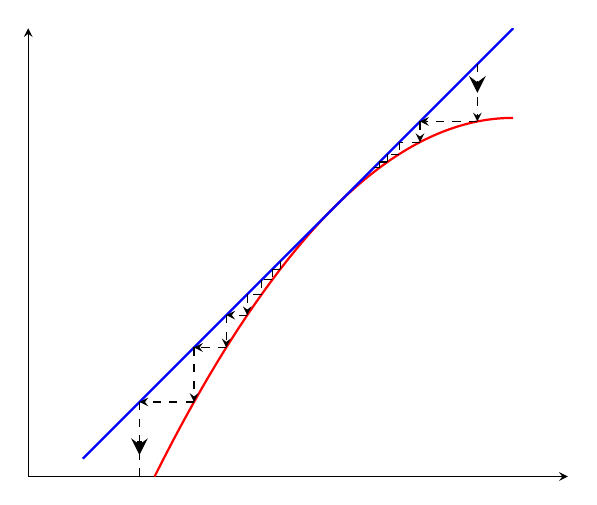
\begin{tikzpicture}
                \begin{axis}[
                    axis lines = left,
                    axis equal, % Asegura que los ejes tengan la misma escala
                    xtick=\empty, % Elimina los ticks del eje x
                    ytick=\empty, % Elimina los ticks del eje y,
                    clip=true,
                    enlargelimits=false, % desactiva el espacio adicional alrededor del gráfico
                ]
                
                % Función
                \def\a{-0.1}
                \pgfmathsetmacro{\b}{1/(2*\a) - 1/(4*\a)}
                \addplot[domain=-10:0, samples=100, color=red, thick] {\a*x^2 + \b};
                
                \addplot[domain=-12:0, samples=2, color=blue, thick]{x};
                
                % Trayectoria de la telaraña
                \draw[dashed,  ultra thick, -stealth] (-1,-1.5) -- (-1, -1.8);
                \draw[dashed, -stealth] (-1,-1) -- (-1,-2.6);
                \draw[dashed, -stealth] (-1,-2.6) -- (-2.6,-2.6);
                \draw[dashed, -stealth] (-2.6,-2.6) -- (-2.6,-3.176);
                \draw[dashed] (-2.6,-3.176) -- (-3.176,-3.176);
                \draw[dashed] (-3.176,-3.176) -- (-3.176, -3.508697);
                \draw[dashed] (-3.176, -3.508697) -- (-3.508697, -3.508697);
                \draw[dashed] (-3.508697, -3.508697) -- (-3.508697, -3.73109);
                \draw[dashed] (-3.508697, -3.73109) -- (-3.73109, -3.73109);
                \draw[dashed] (-3.73109, -3.73109) -- (-3.73109, -3.892107);
                \draw[dashed] (-3.73109, -3.892107) -- (-3.892107, -3.892107);
                
                \draw[dashed] (-6.4937, -6.4937) -- (-6.4937, -6.7168);
                \draw[dashed] (-6.4937, -6.7168) -- (-6.7168, -6.7168);
                \draw[dashed] (-6.7168, -6.7168) -- (-6.7168, -7.01156);
                \draw[dashed] (-6.7168, -7.01156) -- (-7.01156, -7.01156);
                \draw[dashed] (-7.01156, -7.01156) -- (-7.01156, -7.4161);
                \draw[dashed] (-7.01156, -7.4161) -- (-7.4161, -7.4161);
                \draw[dashed, -stealth] (-7.4161, -7.4161) -- (-7.4161, -8);
                \draw[dashed, -stealth] (-7.4161, -8) -- (-8,-8);
                \draw[dashed, -stealth] (-8,-8) -- (-8, -8.9);
                \draw[dashed, -stealth] (-8, -8.9) -- (-8.9, -8.9);
                \draw[dashed, -stealth] (-8.9, -8.9) -- (-8.9, -10.421);
                \draw[dashed, -stealth] (-8.9, -10.421) -- (-10.421, -10.421);
                \draw[dashed, -stealth] (-10.421, -10.421) -- (-10.421, -13.3597);
                \draw[dashed,  ultra thick, -stealth] (-10.421, -11.5) -- (-10.421, -11.9);
    
                \end{axis}
            \end{tikzpicture}
            \caption{Caso de $f$ cóncava, $f''(c)<0$.}
        \end{subfigure}
        \caption{Idea intuitiva de la demostración.}
    \end{figure}
    % // TODO: [Criterio de la Segunda Derivada]
    % https://www.um.es/documents/118351/1884002/TFG_HUERTAS+LOPEZ.pdf/d45e121e-e1fd-4251-bca1-5fc44f9b28e0
    \begin{comment}
    \begin{itemize}
        \item \ul{Supongamos $f''(c)>0$}:

        Como $f''$ es continua, $\exists \delta_1\in \bb{R}^+$ tal que si $|x-c|<\delta_1$, entonces $f''(x)>0$. Por tanto, usando que $f''$ mide el crecimiento de $f'$ y que $f'$ es continua, tenemos que $\exists \delta_2\in \bb{R}^+$, $\delta_2<\delta_1$, tal que:
        \begin{itemize}
            \item $|x-c|<\delta_2$, $x<c$, entonces $f'(x)<1$.
            \item $|x-c|<\delta_2$, $x>c$, entonces $f'(x)>1$.
        \end{itemize}
    \end{itemize}
    \end{comment}
\end{proof}

Volvemos a tener en esta ocasión un caso en el que no tenemos nada que asegurar. Tratamos a su vez de estudiar este caso, con la siguiente proposición:
\begin{prop}[Criterio de la Tercera Derivada]
    Sea la función dada por:
    \Func{f}{I\subseteq \bb{R}}{I\subseteq \bb{R}}{x}{f(x)}
    Supongamos $f \in C^3 (I)$ y sea $x_c \equiv c$ un equilibrio con $f'(c) = 1$ y $f''(c)=0$.
    \begin{itemize}
        \item Si $f'''(c) > 0$, entonces $x_c \equiv c$ es inestable.
        \item Si $f'''(c) < 0$, entonces $x_c \equiv c$ es asintóticamente estable localmente.
    \end{itemize}
\end{prop}
\begin{proof}
Veamos el razonamiento intuitivo con las siguientes gráficas:
    \begin{figure}[H]
        \centering
        \begin{subfigure}{0.4\textwidth}
            \centering
            \begin{tikzpicture}
                \begin{axis}[
                    axis lines = left,
                    axis equal, % Asegura que los ejes tengan la misma escala
                    xtick=\empty, % Elimina los ticks del eje x
                    ytick=\empty, % Elimina los ticks del eje y
                    clip=true,
                    enlargelimits=false, % desactiva el espacio adicional alrededor del gráfico
                ]
                
                % Función
                \addplot[domain=-0.2:2.2, samples=100, color=red, thick] {x^3-3*x^2+4*x-1};
                
                \addplot[domain=-2:2.3, samples=2, color=blue, thick]{x};
                
                % Trayectoria de la telaraña
                
                \draw[dashed, -stealth] ( 0.50000, 0.50000) -- ( 0.50000, 0.37500);
                \draw[dashed, -stealth] ( 0.50000, 0.37500) -- ( 0.37500, 0.37500);
                \draw[dashed, -stealth] ( 0.37500, 0.37500) -- ( 0.37500, 0.13086);
                \draw[dashed, -stealth] ( 0.37500, 0.13086) -- ( 0.13086, 0.13086);
                \draw[dashed, -stealth] ( 0.13086, 0.13086) -- ( 0.13086,-0.52569);
                \draw[dashed, -stealth] ( 0.13086,-0.52569) -- (-0.52569,-0.52569);
                \draw[dashed, -stealth] (-0.52569,-0.52569) -- (-0.52569,-4.07712);
                \draw[dashed,  ultra thick, -stealth] (-0.52569, -1.3) -- (-0.52569, -1.5);
                
                \draw[dashed, -stealth] ( 1.50000, 1.50000) -- ( 1.50000, 1.62500);
                \draw[dashed, -stealth] ( 1.50000, 1.62500) -- ( 1.62500, 1.62500);
                \draw[dashed, -stealth] ( 1.62500, 1.62500) -- ( 1.62500, 1.86914);
                \draw[dashed, -stealth] ( 1.62500, 1.86914) -- ( 1.86914, 1.86914);
                \draw[dashed, -stealth] ( 1.86914, 1.86914) -- ( 1.86914, 2.52569);
                \draw[dashed, -stealth] ( 1.86914, 2.52569) -- ( 2.52569, 2.52569);
                \draw[dashed, -stealth] ( 2.52569, 2.52569) -- ( 2.52569, 6.07712);
                \draw[dashed,  ultra thick, -stealth] (2.52569, 3.3) -- (2.52569, 3.5);
    
                \end{axis}
            \end{tikzpicture}
            \caption{\centering Caso de $f'''(c)>0$.\newline Paso de cóncava a convexa.}
        \end{subfigure}\hfill
        \begin{subfigure}{0.4\textwidth}
            \centering
            \begin{tikzpicture}
                \begin{axis}[
                    axis lines = left,
                    xtick=\empty, % Elimina los ticks del eje x
                    ytick=\empty, % Elimina los ticks del eje y
                    clip=true,
                    enlargelimits=false, % desactiva el espacio adicional alrededor del gráfico
                ]
                
                % Función
                \addplot[domain=0.2:1.8, samples=100, color=red, thick] {-x^3+3*x^2-2*x+1};
                
                \addplot[domain=0.2:1.8, samples=2, color=blue, thick]{x};
                
                % Trayectoria de la telaraña
                \draw[dashed, ultra thick, -stealth] ( 0.5, 0.45) -- ( 0.5, 0.5);
                \draw[dashed, -stealth] ( 0.50000, 0.50000) -- ( 0.50000, 0.62500);
                \draw[dashed, -stealth] ( 0.50000, 0.62500) -- ( 0.62500, 0.62500);
                \draw[dashed, -stealth] ( 0.62500, 0.62500) -- ( 0.62500, 0.67773);
                \draw[dashed] ( 0.62500, 0.67773) -- ( 0.67773, 0.67773);
                \draw[dashed] ( 0.67773, 0.67773) -- ( 0.67773, 0.71120);
                \draw[dashed] ( 0.67773, 0.71120) -- ( 0.71120, 0.71120);
                \draw[dashed] ( 0.71120, 0.71120) -- ( 0.71120, 0.73529);
                \draw[dashed] ( 0.71120, 0.73529) -- ( 0.73529, 0.73529);

                \draw[dashed, ultra thick, -stealth] ( 1.5, 1.55) -- ( 1.5, 1.5);
                \draw[dashed, -stealth] ( 1.50000, 1.50000) -- ( 1.50000, 1.37500);
                \draw[dashed, -stealth] ( 1.50000, 1.37500) -- ( 1.37500, 1.37500);
                \draw[dashed, -stealth] ( 1.37500, 1.37500) -- ( 1.37500, 1.32227);
                \draw[dashed, -stealth] ( 1.37500, 1.32227) -- ( 1.32227, 1.32227);
                \draw[dashed, -stealth] ( 1.32227, 1.32227) -- ( 1.32227, 1.28880);
                \draw[dashed, -stealth] ( 1.32227, 1.28880) -- ( 1.28880, 1.28880);
                \draw[dashed, -stealth] ( 1.28880, 1.28880) -- ( 1.28880, 1.26471);
                \draw[dashed, -stealth] ( 1.28880, 1.26471) -- ( 1.26471, 1.26471);
    
                \end{axis}
            \end{tikzpicture}
            \caption{\centering Caso de $f'''(c)<0$.\newline Paso de convexa a cóncava.}
        \end{subfigure}
        \caption{Idea intuitiva de la demostración.}
    \end{figure}
    En el caso de que $f'''(c)>0$, tenemos que se trata de un punto inflexión que pasa de cóncava a convexa. Por tanto, $\exists\delta\in \bb{R}^+$ tal que:
    \begin{itemize}
        \item $|x-c|<\delta$, $x<c$, entonces $f(x)$ es cóncava. Debido al criterio de la Segunda Derivada, $x_c$ es inestable por abajo.
        \item $|x-c|<\delta$, $x>c$, entonces $f(x)$ es convexa. Debido al criterio de la Segunda Derivada, $x_c$ es inestable por arriba.
    \end{itemize}
    Por tanto, concluimos que $x_c$ es inestable.\\

    En el caso de que $f'''(c)<0$, tenemos que se trata de un punto inflexión que pasa de convexa a cóncava. Por tanto, $\exists\delta\in \bb{R}^+$ tal que:
    \begin{itemize}
        \item $|x-c|<\delta$, $x<c$, entonces $f(x)$ es convexa. Debido al criterio de la Segunda Derivada, $x_c$ es asintóticamente estable por debajo.
        \item $|x-c|<\delta$, $x>c$, entonces $f(x)$ es cóncava. Debido al criterio de la Segunda Derivada, $x_c$ es asintóticamente estable por encima.
    \end{itemize}
    Por tanto, concluimos que $x_c$ es asintóticamente estable localmente.
\end{proof}

Nuevamente surge la pregunta de qué hacer cuando $f'''(c)=0$. Para no alargar más el asunto, pararemos aquí, informando de que en este caso se debería actuar de forma similar, suponiendo que $f\in C^4(I)$ y aplicando criterios de concavidad y convexidad en $c$ para $f$.
También hemos de tener en cuenta que, antes de recurrir al estudio analítico de puntos fijos,
es aconsejable (y muy habitual) dibujar la gráfica de la función y observar el comportamiento
de las órbitas de puntos cercanos al punto fijo.\vspace{1cm}

Recordamos que el Criterio de la Primera Derivada no aportaba información si $|f'(c)|=1$. Ya hemos estudiado con criterios de derivadas de orden mayor si $f'(c)=1$. Estudiaremos ahora el caso de $f'(c)=1$, y para ello emplearemos el siguiente lema.
\begin{lema} \label{lema:f2siif}
    Sea una función $f:I\rightarrow I$ continua, con $I\subset \bb{R}$, y sea su ecuación en diferencias $x_{n+1}=f(x_n)$.
    Un equilibrio $x_c \equiv c$ de la ecuación en diferencias es asintóticamente estable localmente si, y sólo si $x_c\equiv c$ es asintóticamente estable localmente para la ecuación en diferencias $x_{n+1} = (f \circ f)(x_n)$.
\end{lema}
\begin{proof}
    Demostramos por doble implicación:
    \begin{description}
        \item[$\Longrightarrow)$] Supongamos que $x_c$ es asintóticamente localmente estable para $f$. Entonces, por ser estable para $f$, tenemos que:
        \begin{equation*}
            \forall \veps \in \bb{R}^+ \quad \exists \delta \in \bb{R}^+ \mid |x_0-c| < \delta \Longrightarrow |x_n=f^n(x_0)-c|<\veps \qquad \forall n\in \bb{N}
        \end{equation*}

        Por tanto, si esto ocurre para todo $n\in \bb{N}$, en particular ocurre para los múltiplos de $2$, por lo que es estable para $f^2$. Además, por ser un atractor local para $f$, tenemos que:
        \begin{equation*}
            \exists \delta \in \bb{R}^+ \text{ tal que } \left\{\begin{array}{c}
                x_0\in I \\ \land \\ |x_0-c| < \delta
            \end{array}\right\} \Longrightarrow \lim_{n \to \infty} x_n = \lim_{n \to \infty} f^n(x_0)= c
        \end{equation*}

        De igual forma,  si esto ocurre para todo $n\in \bb{N}$, en particular ocurre para los múltiplos de $2$, por lo que es un atractor local para $f^2$. Por tanto, tenemos que es asintóticamente estable localmente para $f^2$.

        \item[$\Longleftarrow)$] Supongamos que $x_c$ es asintóticamente estable localmente para $f^2$. Entonces, por ser estable para $f^2$, tenemos que:
        \begin{equation*}
            \forall \veps \in \bb{R}^+ \quad \exists \delta \in \bb{R}^+ \mid |x_0-c| < \delta \Longrightarrow |x_n=f^{2n}(x_0)-c|<\veps \qquad \forall n\in \bb{N}
        \end{equation*}
        Por tanto, ya está resuelto para las iteradas pares. Para las iteradas impares, buscamos aplicarle la estabilidad a $f(x_0)$, y para ello necesitamos que se tenga que $|f(x_0)-c|<\delta$. Usando la continuidad de $f$ en $c$, fijado $\veps_1=\min\{\nicefrac{\veps}{2},\nicefrac{\delta}{2}\}$ podemos encontrar $\delta_1\in \bb{R}^+$ tal que:
        \begin{equation*}
            |x_0-c|<\delta_1 \Longrightarrow |f(x_0)-f(c)| = |f(x_0)-c|<\veps_1< \delta
        \end{equation*}
        Por tanto, tenemos que:
        \begin{equation*}
            |f^{2n+1}(x_0)-c| = |f^{2n}(f(x_0))-c| < \veps
        \end{equation*}

        Por tanto, como ocurre tanto para las iteradas pares como para las impares, es estable para $f$. Además, por ser un atractor local para $f^2$, tenemos que:
        \begin{equation*}
            \exists \delta \in \bb{R}^+ \text{ tal que } \left\{\begin{array}{c}
                x_0\in I \\ \land \\ |x_0-c| < \delta
            \end{array}\right\} \Longrightarrow \lim_{n \to \infty} x_n = \lim_{n \to \infty} f^{2n}(x_0)= c
        \end{equation*}

        Análogamente al caso anterior, llegamos sin problema a que:
        \begin{equation*}
            \lim_{n \to \infty} f^{2n+1}(x_0) = \lim_{n \to \infty} f^{2n}(f(x_0))= c
        \end{equation*}

        Por tanto, vemos que $x_c$ es asintóticamente estable para $f$.
    \end{description}
\end{proof}

\begin{observacion}
    Nótese que, mediante una sencilla inducción en las hipótesis de la proposición anterior, puede probarse que, para todo $n\in \bb{N}$, se tiene que $x_c \equiv c$ es un equilibrio de la ecuación en diferencias $x_{n+1} = f(x_n)$ es asintóticamente estable localmente si, y sólo si $x_c \equiv c$ es asintóticamente estable localmente para la ecuación en diferencias dada por $x_{n+1} = f^{(2^n)}(x_n)$.
\end{observacion}
\begin{proof}
    Notemos que el caso $n = 0$ es obvio. Procedemos mediante inducción:
    \begin{itemize}
        \item \ul{Caso $n = 1$:}
        Por la proposición anterior, tenemos que es cierto:
        \begin{equation*}
            x_{n+1} = f^{(2^1)}(x_n) = (f \circ f)(x_n) 
        \end{equation*}

        \item \ul{Supuesto que se cumple para $n-1$, probémoslo para $n$:}
        Sabemos por hipótesis de inducción que $x_c \equiv c$ es un equilibrio asintóticamente estable localmente de la ecuación en diferencias $x_{n+1} = f(x_n)$ si, y sólo si lo es para la ecuación en diferencias:
        \begin{equation*}
            x_{n+1} = f^{(2^{n-1})}(x_n) = \overbrace{f \circ \ldots \circ f}^{2^{n-1}}(x_n)
        \end{equation*}
        Sea $g = f^{(2^{n-1})}$ y aplicando el caso $n = 1$, tenemos que dicho equilibrio es asintóticamente estable localmente para la ecuación anterior si, y sólo si lo es para:
        \begin{equation*}
            x_{n+1} = (g \circ g)(x_n) = (\overbrace{f \circ \ldots \circ f}^{2^{n-1}} \circ \overbrace{f \circ \ldots \circ f}^{2^{n-1}})(x_n)
        \end{equation*}
        La composición de $f$ se realiza $2^{n-1} + 2^{n-1} = 2\cdot 2^{n-1} = 2^n$ veces, luego se tiene que:
        \begin{equation*}
            x_{n+1} = (\overbrace{f \circ \ldots \circ f}^{2^{n-1}} \circ \overbrace{f \circ \ldots \circ f}^{2^{n-1}})(x_n) = (\overbrace{f \circ \ldots \circ f}^{2^n})(x_n) = f^{(2^n)}(x_n)
        \end{equation*}
        Tal y como queríamos probar.
    \end{itemize}
\end{proof}

\begin{observacion}
    Notemos además que, si $x_c$ es un equilibrio para $f$, implica que lo es para $f^2$. No obstante, el recíproco no tiene por qué ser cierto, como el caso de que $f$ tenga un $2-$ciclo.
\end{observacion}

~\vspace{1cm}

Llegado este momento, estudiamos entonces el caso de $f'(c)=-1$.
\begin{prop}
    Sea la función dada por:
    \Func{f}{I\subseteq \bb{R}}{I\subseteq \bb{R}}{x}{f(x)}
    Supongamos $f \in C^3 (I)$ y sea $x_c \equiv c$ un equilibrio con $f'(c)=-1$.
    \begin{itemize}
        \item Si $2f'''(c)+3(f''(c))^2 > 0$, entonces $x_c \equiv c$ es asintóticamente estable localmente.
        \item Si $2f'''(c)+3(f''(c))^2 < 0$, entonces $x_c \equiv c$ es inestable.
        \item Si $2f'''(c)+3(f''(c))^2 = 0$, entonces no podemos asegurar nada.
    \end{itemize}
\end{prop}
\begin{proof}
    Consideramos $g=f^2$, y sabemos que $f\in C^3(I)$. Aplicando la regla de la cadena tenemos que, para todo $x\in I$:
    \begin{align*}
        g'(x)&= f(f(x))' = f'(f(x))\cdot f'(x)\\
        g''(x)&= f''(f(x))\cdot (f'(x))^2 + f'(f(x))\cdot f''(x) \\
        g'''(x)&= f'''(f(x))\cdot (f'(x))^3 + 2f'(x)f''(x)\cdot f''(f(x)) + f''(f(x)))f'(x)\cdot f''(x) + f'''(x)\cdot f'(f(x)) =\\
        &= f'''(f(x))\cdot (f'(x))^3 + 3f'(x)f''(x)\cdot f''(f(x)) + f'''(x)\cdot f'(f(x))
    \end{align*}

    Por tanto, evaluando en $c$, tenemos que:
    \begin{align*}
        g'(c) &= f'(c)\cdot f'(c) = 1\\
        g''(c) &= f''(c) - f''(c) = 0\\
        g'''(c) &= -f'''(c) -(3f''(c))^2 -f'''(c) = -\left(2f'''(c) + 3(f''(c))^2\right)
    \end{align*}

    Como $g(c)=f^2(c)=f(c)=c$, $g'(c)=1$, $g''(c)=0$, estamos en condiciones de aplicar el Criterio de la Tercera Derivada para $g$. De esta forma:
    \begin{itemize}
        \item Si $g'''(c)>0$, entonces $x_c$ es inestable para $g$, es decir, no se tiene la estabilidad para los términos pares de la sucesión $\{x_n\}$ asociada a $f$. Por tanto, al o tenerse para los términos pares, podemos asegurar que $x_c$ es inestable para $f$.
        
        \item Si $g'''(c)<0$, entonces $x_c$ es asintóticamente estable para $g$. Por el Lema anterior (Lema \ref{lema:f2siif}), tenemos que $x_c$ es asintóticamente estable para $f$.
    \end{itemize}

    Debido al valor de $g'''(c)$, se deduce directamente lo buscado.
\end{proof}
\begin{observacion} \label{obs:polinomio2grado}
    Sea $f$ un polinomio de grado $2$ la función asociada a una ecuación en diferencias, que es claro que $f \in C^3(I)$. Supongamos que $x_c \equiv c$ es un equilibrio con $f'(c) = -1$. Tenemos que:
    \begin{equation*}
        2f'''(c) + 3(f''(c))^2 = 3(f''(c))^2 > 0
    \end{equation*}
    Entonces, $x_c \equiv c$ es asintóticamente estable localmente.
\end{observacion}

\subsection{Estabilidad de soluciones periódicas. Ciclos}

Sea $x_{n+1} = f(x_n)$ una ley de recurrencia. Recordamos que un $n-$ciclo se determina encontrando los puntos fijos de $f^n$. Además, que no existe ningún $k \in \{1, \ldots, n-1\}$ tal que dicho $n-$ciclo genere un $k-$ciclo. A lo largo de esta sección, debido al trabajo intensivo que realizaremos con ciclos, notaremos un $m-$ciclo como $\{\ol{x_0}, \ldots, \ol{x_{m-1}}\}$

\begin{definicion}[Iterada $k-$ésima]
    Sea $x_{n+1} = f(x_n)$ una ley de recurrencia con $f$ su función asociada, definimos la iterada $k-$ésima de $f$ como la función $f^k$, con $k \in \bb{N}\setminus \{0\}$.
\end{definicion}
Notemos que, si $\{\ol{x_0}, \ldots, \ol{x_{m-1}}\}$ es un $m-$ciclo de la ley de recurrencia dada por $x_{n+1} = f(x_n)$ entonces, $x_c = \ol{x_k}$ es un punto fijo de la iterada $(m\cdot n)-$ésima de $f$, con $n\in \bb{N}\cup \{0\}$. Es decir:
$$\ol{x_k} = f^{n\cdot m} (\ol{x_k}) = f^{n\cdot m+k} (\ol{x_0}) \qquad \forall n\in \bb{N}\cup \{0\}$$

\begin{definicion}[Estabilidad de un $m-$ciclo]
    Sea $x_{n+1} = f(x_n)$ una ley de recurrencia y sea $\{\ol{x_0}, \ldots, \ol{x_{m-1}}\}$ un $m-$ciclo. Diremos que es estable si:
    \begin{multline*}
        \forall \veps\in \bb{R}^+\quad \exists \delta \in \bb{R}^+ \mid |x_k-\ol{x_k}| < \delta \Longrightarrow |f^{m\cdot n+k}(x_0)-\ol{x_k}|<\veps \\ \forall n\in \bb{N}\cup\{0\},~\forall k\in \{0,\dots,m-1\}
    \end{multline*}
    Es decir, es necesario que todos los puntos fijos de la iterada $m-$ésima (los elementos del $m-$ciclo) sean estables para $f^m$, cada uno con su $\delta_k$ asociado. Bastará tomar $\delta=\min\limits_{k}\delta_k$ para obtener lo escrito en la definición anterior.
\end{definicion}

\begin{definicion}[$m-$ciclo localmente atractor]
    Sea $x_{n+1} = f(x_n)$ una ley de recurrencia y sea $\{\ol{x_0}, \ldots, \ol{x_{m-1}}\}$ un $m-$ciclo. Diremos que es localmente atractor si:
    \begin{equation*}
        \exists \delta \in \bb{R}^+ \mid |x_k-\ol{x_k}| < \delta \Longrightarrow \lim_{n\to \infty} f^{m\cdot n+k}(x_0) = \ol{x_k} \qquad \forall k\in \{0,\dots,m-1\}
    \end{equation*}
    Es decir, es necesario que todos los puntos fijos de la iterada $m-$ésima (los elementos del $m-$ciclo) sean atractores locales para $f^m$, cada uno con su $\delta_k$ asociado. Bastará tomar $\delta=\min\limits_{k}\delta_k$ para obtener lo escrito en la definición anterior.
\end{definicion}

\begin{definicion}[$m-$ciclo asintóticamente localmente estable]
    Sea $x_{n+1} = f(x_n)$ una ley de recurrencia y sea $\{\ol{x_0}, \ldots, \ol{x_{m-1}}\}$ un $m-$ciclo. Diremos que es asintóticamente localmente estable si es estable y además es atractor local.
\end{definicion}

No obstante, al igual que en el caso de los puntos de equilibrio, tenemos un importante criterio para analizar la estabilidad asintótica sin necesidad de emplear la definición formal.
\begin{teo}
    Sea $f:I\rightarrow I$, $I \subseteq \bb{R}$, $f \in C^1(I)$ y $\{\ol{x_0}, \ldots, \ol{x_{m-1}}\}$ un $m-$ciclo para $x_{n+1} = f(x_n)$. Entonces:
    \begin{itemize}
        \item Si $|f'(\ol{x_0})\cdot f'(\ol{x_1})\cdot \ldots \cdot f'(\ol{x_{m-1}})| < 1$ entonces, el $m-$ciclo es asintóticamente estable localmente.
        \item Si $|f'(\ol{x_0})\cdot f'(\ol{x_1})\cdot \ldots \cdot f'(\ol{x_{m-1}})| > 1$ entonces, el $m-$ciclo es inestable.
    \end{itemize}
\end{teo}
\begin{proof}
    Veamos que $\ol{x_k}$ es asintóticamente localmente estable para $f^m$. Para calcular $(f^m)'$, demostramos por inducción que, para todo $m\in \bb{N}$, se tiene que:
    \begin{equation*}
        (f^m(x))' = \prod_{k=0}^{m-1} f'(f^k(x)) \qquad \forall x\in I
    \end{equation*}
    donde $f^0(x)=x$.
    \begin{itemize}
        \item \ul{Para $m=2$}:
        \begin{equation*}
            (f^2(x))' = f'(f(x))\cdot f'(x) = \prod_{k=0}^{1} f'(f^k(x))
        \end{equation*}

        \item \ul{Supuesto cierto para $m$, demostramos para $m+1$}:
        \begin{align*}
            (f^{m+1}(x))' &= \left(f(f^m(x)\right)'
            = f'(f^m(x))\cdot (f^m(x))'
            =\\&= f'(f^m(x)) \prod_{k=0}^{m-1} f'(f^k(x))
            = \prod_{k=0}^{m} f'(f^k(x))
        \end{align*}
    \end{itemize}

    Por tanto, como en ese producto se recorrerá el ciclo completo, tenemos que:
    \begin{equation*}
        (f^m(\ol{x_k}))' = \prod_{j=0}^{m} f'(\ol{x_j})
    \end{equation*}

    Aplicando por tanto el Criterio de la Primera Derivada para $f^m$, se tiene de forma directa.
\end{proof}

\section{Modelo logístico}\label{sec:DesarrolloModeloLogistico}

Recordamos que este modelo se presentó en la sección \ref{sec:IntroModeloLogistico}, motivado por evitar el crecimiento ilimitado o la extinción del modelo de Malthus. Para evitar la tasa de crecimiento constante, se definía esta como una recta, de la forma:
\begin{equation*}
    \frac{p_{n+1}}{p_n} = a-bp_n \qquad a,b\in \bb{R}
\end{equation*}

De esta forma, se tiene que $p_{n+1}=p_n(a-bp_n)$.
Además, vimos que para este modelo tenga sentido y no haya poblaciones negativas, es necesario que se tenga que $0\leq p_0\leq \nicefrac{a}{b}$, llamada esta última \emph{población tope}. Veamos que haciendo un cierto cambio de variable, este modelo también lo podemos escribir como:
$$x_{n+1} = ax_n(1-x_n)\qquad a\in \bb{R}^+$$
\begin{proof}
    Proponemos realizar el cambio de variable:
    \begin{equation*}
        x_n = \dfrac{p_n}{\nicefrac{a}{b}} = b\cdot \dfrac{p_n}{a}
    \end{equation*}
    De esta forma, tenemos que:
    \begin{align*}
        x_{n+1} &= b\cdot \dfrac{p_{n+1}}{a} = \dfrac{b}{a}\cdot p_n(a-bp_n) = \dfrac{b}{a}\cdot p_n {a}\left(1-\dfrac{b}{a}\cdot p_n\right) = ax_n (1-x_n)
    \end{align*}
\end{proof}

Como ventaja de esta forma de escribirlo, tenemos que es adimensional; ya que $x_n$ es una cantidad sin unidades al serlo $a$ y $bp_n$. Representa por tanto porcentajes de la población, ya que buscamos que $x_n\in [0,1]$ para todo $n\in \bb{N}$:
\begin{itemize}
    \item Si $x_n=0$, implica que no hay individuos en la población.
    \item Si $x_n=1$, implica que la población toma el valor número de individuos, que se ha visto que es la \emph{población tope}, $\nicefrac{a}{b}$.
\end{itemize}

Nos preguntamos ahora qué es necesario para que el modelo esté bien planteado, es decir, que $x_n\in [0,1]$ para todo $n\in \bb{N}$.
\begin{prop}
    Sea un modelo logístico de la forma:
    \begin{equation*}
        x_{n+1} = ax_n (1-x_n)\qquad \text{\ con\ } a\in \bb{R}^+.
    \end{equation*}
    Para que $x_n \in [0,1]\quad \forall n \in \bb{N}$, necesitamos que $a\in ]0,4]$
\end{prop}
\begin{proof}
    Sea la función asociada al modelo logístico,
    \Func{f}{[0,1]}{\bb{R}}{x}{ax(1-x)}

    Tenemos que es derivable, y su único punto crítico es el valor que anula su primera derivada:
    \begin{equation*}
        f'(x)=a(1-x) -ax = 0 \Longleftrightarrow 1-x = x \Longleftrightarrow x=\frac{1}{2}
    \end{equation*}

    Además, tenemos que $f''(x)=-2a<0$, por lo que la función alcanza su máximo absoluto en $x = \dfrac{1}{2}$, con valor $f\left(\dfrac{1}{2}\right) = \dfrac{a}{4}$.
    Para conseguir que $f([0,1]) \subseteq [0,1]$, exigimos:
    \begin{equation*}
        f\left(\dfrac{1}{2}\right) = \dfrac{a}{4} \leq 1 \Longleftrightarrow a \leq 4
    \end{equation*}

    Por tanto, tenemos que $0<a\leq 4$, por lo que $a\in ]0,4]$ y se tiene lo pedido.
\end{proof}

La anterior proposición se ve claramente en la siguiente Figura, ya que para valores mayores que $4$ se tiene que $f(x)\not\subset [0,1]$.
\begin{figure}[H]
    \centering
    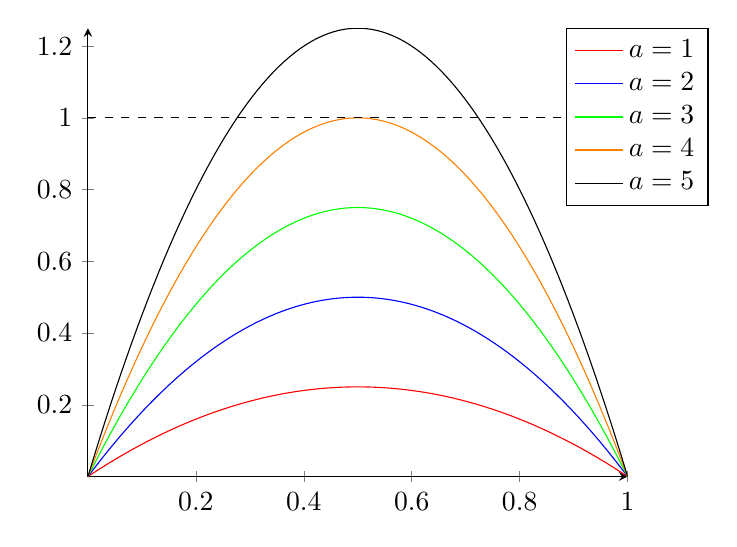
\begin{tikzpicture}
        \begin{axis}[
            axis lines=center,
            legend style={at={(1.15,1)}, anchor=north east}, % Posición de la leyenda
        ]
        
        % Funciones
        \addplot[domain=0:1, samples=100, color=red]{1*x*(1-x)};
        \addplot[domain=0:1, samples=100, color=blue]{2*x*(1-x)};
        \addplot[domain=0:1, samples=100, color=green]{3*x*(1-x)};
        \addplot[domain=0:1, samples=100, color=orange]{4*x*(1-x)};
        \addplot[domain=0:1, samples=100, color=black]{5*x*(1-x)};

        % Recta y=1
        \addplot[domain=0:1, samples=2, dashed] {1};
        
        % Leyenda
        \legend{$a=1$, $a=2$, $a=3$, $a=4$, $a=5$}
        \end{axis}
    \end{tikzpicture}
    \caption{\centering Modelo logístico, $f(x)=ax(1-x)$ para distintos valores de $a$.}
\end{figure}

Ahora, trataremos de buscar soluciones del modelo logístico. Comenzamos por lo que nos es más natural, estudiar primero los puntos fijos del modelo.
\subsection{Puntos fijos}
Estudiando los puntos fijos de la función $f(x) = ax(1-x)$, tenemos que:
\begin{equation*}
    c = ac(1-c) \Longrightarrow
    \left\{\begin{array}{l}
        c_1=0\\
        \lor \\
        1 = a-ac_2 \Longrightarrow c_2 = \frac{a-1}{a}
    \end{array}\right.
\end{equation*}
Notemos que la segunda solución constante no tiene sentido biológico (poblacional) si $a\in [0,1]$.\\

Estudiemos ahora la estabilidad de dichas soluciones constantes. Tenemos que la función asociada al modelo logístico es $f(x) = ax(1-x)$, derivable con:
\begin{equation*}
    f'(x) = a-2ax
\end{equation*}

Sustituyendo en las soluciones constantes, y aplicando el Criterio de la Primera Derivada, obtenemos que:
\begin{equation*}
    f'(0) = a \Longrightarrow \left\{ \begin{array}{ll}
        \text{Si\ } a<1 & \text{entonces, es asintóticamente estable localmente} \\
        \text{Si\ } a>1 & \text{entonces, es inestable}
    \end{array} \right.
\end{equation*}
\begin{equation*}
    f'\left(\dfrac{a-1}{a}\right) = 2-a \Rightarrow \left\{ \begin{array}{ll}
         \text{Si\ } 1 < a < 3 & \text{entonces, es asintóticamente estable localmente} \\
         \text{Si\ } a > 3 & \text{entonces, es inestable}
    \end{array}\right.
\end{equation*}

Nos queda por tanto estudiar los casos $a = 1$ para $x_0$ y $a = 3$ para $x_{\frac{a-1}{a}}$:
\begin{itemize}
    \item \ul{$a = 1$}: En este caso solo hay una solución constante, $x_c=0$. Tenemos que:
    \begin{equation*}
        f'(0) = 1 \qquad
        f''(x) = -2a < 0
    \end{equation*}

    Aplicando el Criterio de la Segunda Derivada, obtenemos que $x_c \equiv 0$ es asintóticamente estable localmente por arriba e inestable por abajo. Como el modelo está definido en $[0,1]$, tan solo nos interesa lo que ocurre por encima del $0$, por lo que lo consideramos asintóticamente localmente estable.

    \item \ul{$a=3$:}
    \begin{equation*}
        f'\left(\dfrac{a-1}{a}\right) = -1
    \end{equation*}
    Por la observación de la página \pageref{obs:polinomio2grado}, tenemos que es asintóticamente estable localmente.
\end{itemize}

En resumen, tenemos el siguiente resultado, donde \emph{a.e.l.} representa \emph{asintóticamente estable localmente}.
\begin{table}[H]
    \centering
    \begin{tabular}{c|l}
        $0< a \leq 1$ & $0$ es a.e.l.\\ \hline
        $1<a\leq 3$ & $0$ es inestable y $\frac{a-1}{a}$ es a.e.l.\\ \hline
        $3<a\leq 4$ & $0$ y $\frac{a-1}{a}$ son inestables.
    \end{tabular}
\end{table}